%% LaTeX2e class for student theses
%% thesis.tex
%% 
%% Karlsruhe Institute of Technology
%% Institute for Program Structures and Data Organization
%% Chair for Software Design and Quality (SDQ)
%%
%% Dr.-Ing. Erik Burger
%% burger@kit.edu
%%
%% Version 1.3.2, 2017-08-01

%% Available page modes: oneside, twoside
%% Available languages: english, ngerman
%% Available modes: draft, final (see README)
\documentclass[twoside, english]{sdqthesis}

\usepackage[nonumberlist]{glossaries}
\usepackage{tabularx}
\usepackage{makecell}
\usepackage{pdflscape}
\usepackage{pifont}% http://ctan.org/pkg/pifont
\newcommand{\cmark}{\ding{51}}%\\
\usepackage{adjustbox}

\renewcommand\theadfont{\bfseries}
\renewcommand\theadgape{\Gape[3pt]}
\renewcommand\cellgape{\Gape[3pt]}

\makeglossaries
\newglossaryentry{EMS}{%
	name={EMS},%
	description={Emergency Medical Services}%
}

\newglossaryentry{EMG}{%
	name={EMG},%
	description={Electromyography}%
}

\newglossaryentry{CPR}{%
	name={CPR},%
	description={Cardiopulmonary Resuscitation}%
}

\newglossaryentry{BVM}{%
	name={BVM},%
	description={Bag-Valve-Mask}%
}

\newglossaryentry{HAR}{%
	name={HAR},%
	description={Human Activity Recognition}%
}

\newglossaryentry{SMA}{%
	name={SMA},%
	description={Signal Magnitude Area}%
}

\newglossaryentry{RMS}{%
	name={RMS},%
	description={Root Mean Square}%
}

%% ---------------------------------
%% | Information about the thesis  |
%% ---------------------------------

%% Name of the author
\author{David Greiner}

%% Title (and possibly subtitle) of the thesis
\title{Wearable sensors for automatic detection of trauma procedures}

%% Type of the thesis 
\thesistype{Master's Thesis}

%% Change the institute here, ``IPD'' is default
\myinstitute{Institute for Anthropomatics and Robotics}

%% You can put a logo in the ``logos'' directory and include it here
%% instead of the SDQ logo
\grouplogo{OSU_horizontal_2C_O_over_B}
%% Alternatively, you can disable the group logo
% \nogrouplogo

%% The reviewers are the professors that grade your thesis
\reviewerone{Prof. Dr. U. Hanebeck}
\reviewertwo{Prof. }

%% The advisors are PhDs or Postdocs
\advisorone{Prof. Dr. Julie A. Adams}
%% The second advisor can be omitted
\advisortwo{M.Sc. Jamison Heard}

%% Please enter the start end end time of your thesis
\editingtime{January 14th, 2018}{July 14th, 2018}

\settitle

%% --------------------------------
%% | Settings for word separation |
%% --------------------------------

%% Describe separation hints here.
%% For more details, see 
%% http://en.wikibooks.org/wiki/LaTeX/Text_Formatting#Hyphenation
\hyphenation{
% me-ta-mo-del
}

%% --------------------------------
%% | Bibliography                 |
%% --------------------------------

%% Use biber instead of BibTeX, see README
\usepackage[citestyle=numeric,style=numeric,backend=biber,maxbibnames=99,doi=false,isbn=false,url=false,firstinits=false]{biblatex}
\addbibresource{thesis.bib}

%% ====================================
%% ====================================
%% ||                                ||
%% || Beginning of the main document ||
%% ||                                ||
%% ====================================
%% ====================================
\begin{document}

%% Set PDF metadata
\setpdf

%% Set the title
\maketitle

%% The Preamble begins here
\frontmatter

%% LaTeX2e class for student theses: Declaration of independent work
%% sections/declaration.tex
%% 
%% Karlsruhe Institute of Technology
%% Institute for Program Structures and Data Organization
%% Chair for Software Design and Quality (SDQ)
%%
%% Dr.-Ing. Erik Burger
%% burger@kit.edu
%%
%% Version 1.3.2, 2017-08-01

\thispagestyle{empty}
\null\vfill
\noindent\hbox to \textwidth{\hrulefill} 
\iflanguage{english}{I declare that I have developed and written the enclosed
thesis completely by myself, and have not used sources or means without
declaration in the text.}%
{Ich versichere wahrheitsgemäß, die Arbeit
selbstständig angefertigt, alle benutzten Hilfsmittel vollständig und genau
angegeben und alles kenntlich gemacht zu haben, was aus Arbeiten anderer
unverändert oder mit Änderungen entnommen wurde.}
 
 
%% ---------------------------------------------
%% | Replace PLACE and DATE with actual values |
%% ---------------------------------------------
\textbf{PLACE, DATE}
\vspace{1.5cm}
 
\dotfill\hspace*{8.0cm}\\
\hspace*{2cm}(\theauthor) 
\cleardoublepage

\setcounter{page}{1}
\pagenumbering{roman}

%% ----------------
%% |   Abstract   |
%% ----------------
 
%% For theses written in English, an abstract both in English
%% and German is mandatory.
%%
%% For theses written in German, a German abstract is sufficient.
%%
%% The text is included from the following files:
%% - sections/abstract

\includeabstract

%% ------------------------
%% |   Table of Contents  |
%% ------------------------
\tableofcontents

\listoffigures
\listoftables
\printglossary[style=long]

%% -----------------
%% |   Main part   |
%% -----------------

\mainmatter

%% LaTeX2e class for student theses
%% sections/problem_statement.tex
%% 
%% Karlsruhe Institute of Technology
%% Institute for Program Structures and Data Organization
%% Chair for Software Design and Quality (SDQ)
%%
%% Dr.-Ing. Erik Burger
%% burger@kit.edu
%%
%% Version 1.3.2, 2017-08-01

\chapter{Problem Statement}
\label{ch:Problem-Statement}

Treating a person with severe trauma is extremely challenging, as the injury may result in life-threatening effects on blood circulation and tissue oxygenation. Every decision can make the difference between life and death. After the first assessment by the emergency medical services (\gls{EMS}), the patient's medical state has to be continuously monitored. Upon arrival at the hospital, it is important for the trauma team to understand the patient's treatment history, including what medications have been administered and emergency procedures have been performed. This information is vital to providing the most accurate and beneficial care; however, such life-critical information may not be properly communicated when transferring the patient from the \gls{EMS} personnel's care to the hospital trauma team. \gls{EMS} personnel often rely on their memory to communicate the patient's treatment history, which can be inaccurate. Failing to communicate a complete and accurate treatment history can lead to permanent damage or death. This thesis proposes an automatic reporting system using accelerometer, gyroscope, and electromyography (\gls{EMG}) data to detect a subset of common procedures performed on trauma patients. An algorithm that incorporates machine-learning will be developed to classify the subset of \gls{EMS} procedures based on the wearable sensor data.
\par Automatically detecting trauma procedures may improve the communication during the care transfer between EMS personnel and the trauma team. Some ambulances are equipped with devices that record the patient's vitals and statistics about cardiopulmonary resuscitation (\gls{CPR}), such as the duration, frequency, and depth of the chest compressions. Missing from these devices is the ability to automatically detect other common EMS procedures. Information about the patient's care is typically entered into the patient's transcript after completing the patient hand-off to the trauma team. When arriving at the hospital, paramedics can provide records e.g., graphs and vital statistics, on a tablet, in addition to the standard oral communication protocol. The full transcript is transmitted via the Internet to the hospital's database when connected to the secured city network. The data transfer usually does not occur until the ambulance arrives back at the station. Currently, transferring patient care information is a slow and static process. Real-time information about the patient's state will be beneficial for the trauma team before the patient arrives at the hospital, as this advanced information knowledge allows the hospital staff to properly prepare the emergency room for the severity of the case.
\par The proposed detection of a subset of commonly performed EMS procedures on trauma patients includes \gls{CPR}, airway management, placing splints, and placing an intravenous (\gls{IV}) line. CPR is the process of helping a person breath using chest compressions and artificial ventilation. Airway management consists of multiple procedures depending on the severity of the trauma. Bag-valve-mask ventilation provides air for patients with breathing difficulties, while an oropharyngeal device is used to manage an unresponsive patient's airway. Oropharyngeal devices keep the tongue from obstructing the airway. Severe trauma patients require intubation, in which a tube is inserted orally and reaches into the windpipe. Splinting stabilizes an extremity that is fractured or broken. An intravenous drip allows for fluids and medication to be administered into the patient’s bloodstream.
\par The EMS procedures are broken into their anatomical movements using hierarchical task analysis, which determined that each EMS procedure requires a specific sequence of anatomical movements. Each sequence will generate patterns in the accelerometer, gyroscope, and EMG data, which the developed task recognition algorithm will be able to detect.
\par A major challenge of detecting a procedure is that the EMS personnel must use two arms to perform the necessary care for the patient. Therefore, each arm must be monitored and both data-sets have to be considered by the automatic task recognition algorithm. A second challenge is that there are individual differences in the body movements when executing EMS procedures. Depending on the EMS personnel, body movements vary from using a different finger to another motion. Another challenge is accounting for an ambulance's abrupt turns, fast acceleration and sudden stops, as such ambulance movements generate noise on the accelerometer and gyroscope data unrelated to the EMS personnel's movement, and must be filtered.
\par Chapter \ref{ch:Literature-Review} provides background information on existing systems to detect physical movement. Chapter \ref{ch:System-Design} proposes an algorithm that detects trauma procedures by \gls{EMS} personnel. Chapter \ref{ch:Experimental-Design} introduces an experimental design for studies to collect data and test the algorithm. Chapter \ref{ch:Results} presents the results of the studies. Finally, Chapter \ref{ch:Conclusion} outlines the contribution and drawbacks of the algorithm, followed by a discussion how future work could improve the system. 
%% LaTeX2e class for student theses
%% sections/literature_review.tex
%% 
%% Karlsruhe Institute of Technology
%% Institute for Program Structures and Data Organization
%% Chair for Software Design and Quality (SDQ)
%%
%% Dr.-Ing. Erik Burger
%% burger@kit.edu
%%
%% Version 1.3.2, 2017-08-01

\chapter{Literature Review}
\label{ch:Literature-Review}

\section{Hand-Off Communication}
\label{sec:Literature-Review:Hand-Off-Communication}
A hand-off in the medical community is the process of transferring a patient from one care provider to another \cite{SoletDJNorvellJMRutanGH2005}. During the hand-off process key information is communicated, e.g., the patient’s state, administered medication, and treatment. The emergency medical service (\gls{EMS}) hand-off process consists of multiple stages. Initially, patient information is communicated to the hospital trauma team during patient transport. Once the patient arrives, and care is transferred from the EMS personnel to the hospital, more detailed information is communicated. Compared to the initial information, the detailed information includes personal data, such as address, insurance information, previous injuries, etc. and a step-by-step list of treatment events. Finally, after the EMS return to the rescue station, a complete report of the patient's treatment is compiled, and the process is complete \cite{Cohen2010}.
\par Inadequate communication is the leading cause of malpractice lawsuits; in 2015, three out of ten malpractice lawsuits mention a breakdown in communication \cite{CRICOStrategies.2015}. Doctors spend most of their time communicating with patients and other care providers. An observation of doctors for 35 hours and 13 minutes found that doctors engaged in communication events 78.7\% of the time \cite{Spencer2004}. When a patient arrives at the hospital, communication between hospital staff can take place in several different ways. Bhabra, Mackeith, Monteiro, and Pothier \cite{Bhabra2007} compared information loss during hand-off for three communication methods: verbal communication, verbal communication with note-taking, and exchange of a printed treatment record by the person handing off the patient to the person assuming the responsibility of care. Every participant received the same communication in every cycle. After five cycles the information loss when communicating verbally was 97.5\%, note-taking by the receiving person incurred a 14.5\% information loss, and handing a printed sheet to the receiving person resulted in 1.25\% information loss \cite{Bhabra2007}. The small information loss during communication using a printed sheet was due to the amount of information a participant had to remember. The only information loss when exchanging a printed sheet occurred during the fifth cycle, while 100\% of the information was retained during all previous cycles. Bhabra et al.’s study focused on in-hospital care transfer and did not consider time critical or trauma situations. A study of hand-offs between EMS personnel and emergency department staff found that the quality of information exchange in the emergency department is higher for trauma patients than for non-trauma patients \cite{Meisel2015}. EMS personnel reported that when handling trauma cases, the emergency department staff were highly engaged and desired a detailed report, while emergency department staff were less interested in non-trauma patients.
\par The Joint Commission on Accreditation of Healthcare Organizations set a goal to improve medical hand-off communication \cite{Arora2006}. The commission conducted a study and found that the hand-off communication process is highly variable and discipline-specific. Therefore, every discipline and department developed a protocol specific to their unique requirements. A study comparing medical errors and preventable adverse events before and after the introduction of a standardized hand-off communication protocol for patient admission at nine pediatric residency training programs in the United States and Canada was conducted. The study found that the medical error rate during the EMS hand-off process decreased by 23\%, and the rate of preventable adverse events decreased by 30\% after the implementation of a standardized hand-off communication protocol \cite{Starmer2014}. An automatic detection system can provide additional information that an \gls{EMS} personnel may have missed, further increasing the reporting accuracy and decreasing the medical error rate.
\par Hand-off communication in nursing is commonly done using an Electronic Health Record. Electronic Health Records store a patient's medical records and allow medical professionals to input vital data and share treatment information. It was determined, that using these systems improved the continuity of care and increased the consistency of data \cite{COLLINS2011704}. The existing Electronic Health Record can be updated using an automatic detection system to provide real-time information regarding a patient's care, from the time the EMS personnel arrive at the scene until the hand-off at the hospital.
\par The hand-off communication between \gls{EMS} personnel and the hospital's team presents unique challenges. Both sets of personnel have different worksites and clinical duties, which may result in communication errors due to the personnel being unfamiliar with each others' procedures. The time window during which the communication occurs is extremely short. Information communication during transport is limited due to the urgency to provide care to the patient. Automatically detecting procedures may augment the verbally communicated information and may be sent in real-time through a different communication modality. Depending on the patient's level of acuity, emergency department staff may pay less attention during the hand-off communication, if the injuries are deemed non-life-threatening \cite{SoletDJNorvellJMRutanGH2005,Meisel2015}. If a patient with a common injury arrives, emergency department staff may assume they already know everything about the case; therefore, potentially missing critical information and resulting in permanent injury or death.

\section{Human Activity Recognition}
\label{sec:Literature-Review:Human-Activity-Recognition}
\emph{Human Activity Recognition} (\gls{HAR}) is a method intended to recognize common human activities in real life settings \cite{Helal2010}. HAR uses patterns discovered from low-level sensor data to train activity models that can be used to detect the human's activity.
\par Increasing interest in HAR has lead to improved computational power, smaller size, and lower cost of sensors \cite{Rodgers2015}. The sensors used to recognize human activities fall into two categories: \emph{external} and \emph{wearable} sensors \cite{Lara2013}. An external sensor observes the human from a fixed point of view and relies on human interaction within the sensor's range and field of view. A wearable sensor is worn on the user's body and collects information as the human conducts their activities. The reviewed sensor types and the anticipated associated advantages and disadvantages for automatically detecting EMS procedures are provided in Table \ref{har-sensors}. The following chapter examines the advantages and disadvantages for each sensor and how they can be used to automatically detect EMS procedures.
\begin{table}[]
	\centering
	\caption{Summary of Human Activity Recognition sensors}
	\label{har-sensors}
	\begin{tabularx}{\textwidth}{|c|X|X|}
		\hline
		\thead{Sensor} & \thead{Advantages} & \thead{Disadvantages}  \\\hline
		\makecell{Camera} & \makecell{Captures all body parts of\\the human\\Not worn on the body\\Higher information flow\\Capture information around\\the human} & \makecell{Requires human to be in\\field of view\\Higher privacy invasion\\Computational expensive\\Requires good lighting} \\\hline
		\makecell{Environmental} & \makecell{Senses the environmental\\context of the human} & \makecell{Not very accurate for HAR} \\\hline
		\makecell{Acceleration} & \makecell{Most accurate wearable sensor\\for HAR} & \makecell{Sensor placement can\\make a difference} \\\hline
		\makecell{Location} &\makecell{Useful for detecting\\transportation} & \makecell{Not useful for fine-grained\\detection} \\\hline
		\makecell{Physiological} & \makecell{Useful for measuring human's\\activity load} & \makecell{Activity load is different\\depending on fitness level} \\\hline
	\end{tabularx}
\end{table}

\subsection{External Sensors}
Extensive \gls{HAR} research has focused on using cameras as external sensors to visually recognize gestures and movement. Visual recognition has two primary sources of data: RGB and grayscale video. RGB data is the visual representation of the camera in pixels of red, green, and blue values. Grayscale data is the depth representation of the camera in a shade of gray, white being closest and black being the furthest away. Multiple features can be extrapolated from the video data, e.g., body part detection \cite{Chakraborty2008}, motion detection \cite{4813430}. A common analysis approach uses background subtraction to project a silhouette onto a person, which allows for the detection of a region of interest within which motion occurs \cite{Bobick2001}. Isolating this motion permits a more detailed analysis of the region of interest. Motion around the patient, in the context of an ambulance, indicates that a procedure is likely being performed. Using multiple cameras, it is possible to generate 3D models with silhouettes of humans \cite{Weinland2006}. 3D models are used to generate information regarding the positioning of human limbs, the human's distance relative to other objects, and the human's pose.
\par Regions of interest can be detected using motion information in the video. The difference between video frames is analyzed pixel-wise to determine the direction of the movement, making it useful for detecting moving objects when the camera is steady \cite{Efros03}. Humans are rarely stationary; therefore the motion information can be used to generate features, such as the human's speed.
\par Joint angle detection is more complex than detecting silhouettes. Joint detection provides a richer dataset to a HAR algorithm, which can increase the algorithm’s accuracy \cite{CGV-005}. Joint detection requires a 3D scene to maintain a representation that is view-invariant \cite{Poppe2010}. Using joints and their angles allows for reconstructing and identifying the human skeleton. Understanding the human skeletal position allows for more accurate classifications of skeletal-based human activities, such as waving an arm, jumping, or sitting \cite{HsuanSheng}.

\subsection{Wearable Sensors}
Wearable sensors come in all shapes and sizes. Most people never notice how many sensors are carried around in their devices on a daily basis. Wearable sensors for human activity recognition fall into one of four groups: environmental attributes, acceleration, location, and physiological signals \cite{Lara2013}. Sensors for environmental attributes do not collect data about the human, but rather about the human's surrounding environment \cite{Juha2006}. A sensor for environmental attributes is the air pressure sensor which measures the altitude of the human \cite{5559476}, or the humidity sensor which measures the amount of amount of water vapor in the air \cite{Qin2007}. An acceleration sensor senses the movement of the body part on which its placed, relative to the whole body movement \cite{Maurer2006}. An acceleration senors may contain up to three axes (X,Y,Z). A popular use for acceleration sensors in smartphones is step counting of the human's activity \cite{Brajdic:2013}. Location sensors determine the location of the human as coordinates on a map \cite{Quddus2003}. For example, a Global Positioning System (GPS) sensor uses satellites in space to triangulate a human's position to latitude, longitude, and elevation \cite{hofmann2012global}. Physiological signals sensors monitor the human's vital signs \cite{Yin:2008}. For example, heart rate, respiration rate, skin temperature, and electrocardiogram amplitude can be used to improve activity recognition \cite{Lara2012}.
\par Environmental attributes relate to the human's surroundings, e.g., temperature, noise level, and light intensity \cite{Maurer2006}. These environmental attributes allow for detecting the climate the human is currently experiencing. For example, using the air pressure an approximate location of the human in a subway system can be determined \cite{van2017subwayapps}. Depending on the environmental attributes, humans may be more likely to take part in certain activities, such as walking in sunshine and warm weather. Environmental attribute information may be insufficient as the sole means of recognizing human activity.
\par The most broadly used HAR sensors are the accelerometer and gyroscope sensors \cite{Lara2013}. The acceleration and gyroscope sensors are commonly found in almost every smart device, e.g., smartphones \cite{5560598}, smartwatches \cite{Shen:2016}, fitness trackers \cite{Kaewkannate2016}. The placement of the sensor on the human body is important for accurately detecting the human's activity, as body parts move differently depending on the activity. For example, movements while sitting cannot be captured if the sensor is placed in the human's pockets \cite{Maurer2006}.
\par Location information is usually obtained using a GPS sensor, which is interesting for moving humans, as their means of transportation can be detected using the human's speed \cite{Zheng2008}. Additionally, the geographical context helps infer the activity in which the human is engaged \cite{liao2006location}. For example, 30\% of traffic in urban areas are due to drivers searching for a parking spot. A system using GPS sensors can detect when a spot has vacated and alert a nearby driver \cite{Nawaz:2013}.
\par Finally, physiological signals, e.g., heart rate, respiration rate, and skin temperature, can be used alongside acceleration data to more accurately predict human activity \cite{Lara2012}. Activities may have different effects on a human's physiological metrics \cite{Lara2013}. For example, the more demanding the activity, the higher the heart-rate and the lower the respiration rate \cite{Lara2013}.
\par Recognizing human activities from wearable sensors requires data acquisition. Data is acquired in multiple stages \cite{Lara2013}. First, wearable sensors are selected for their suitability to detect a certain actions or activities representative of a task. Second, the wearable sensors are integrated with devices that capture the data. Finally, the data is stored either locally on the integration device or remotely on a server. During the data acquisition process subjects perform a predefined set of activities that the recognition system is later able to detect. After the data is collected, activity recognition consists of two stages, training and testing the activity recognition system, which is described in Chapter \ref{sec:Literature-Review:Machine-Learning-Classifiers}.

\subsection{Differences}
External and wearable sensors differ in regards to privacy, pervasiveness, complexity, mobility, and accuracy. These factors are important for developing a system to detect the medical procedures EMS personnel apply to a patient. Privacy is extremely important in a healthcare environment, which is why the United States has HIPAA \cite{HIPAA} and Germany has "Die \"artzliche Schweigepflicht" \cite{Privatgeheimnissen}. Pervasiveness is defined as the sensor's ability to be connected or attached to any device and any location \cite{Lara2013}. Proper functioning of the automatic detection system requires the system must run in real-time. EMS personnel are usually mobile when performing their duties from initiating patient care to transporting and hand-off at the hospital. Finally, sensor accuracy is critical, as a falsely recognized EMS procedure may have fatal results \cite{mourcou2015performance}.
\par Privacy has become a growing societal concern \cite{privacyindex}. Patients and EMS personnel may object to constant monitoring using cameras \cite{Arning2015}. Over 40\% of police leadership think that body-worn cameras are used to "fish" for evidence against their officers \cite{Smykla2016}. The same problem may occur when EMS personnel are equipped or surrounded by cameras, as the video may be used as evidence of wrong-doing. Wearable sensors may reduce this perception of privacy intrusion, as the wearable sensor is a passive observer without the camera.
\par Pervasiveness for external sensors is low, because cameras can not be easily attached to humans. The cameras have to be mounted externally and pointed at the human. The monitored human has to stay within a perimeter defined by the position and the field of view of the camera. Inside an ambulance multiple cameras have to be deployed to mitigate the obscureness effect of body parts covering a region of interest \cite{howe2000bayesian}. Wearable sensors can capture data the entire time the sensor is worn, while cameras collect more informative data concerning the overall environment and activities that wearable sensors may be unable to detect.
\par Video processing is extremely computational expensive; therefore, external sensors have high complexity. A Full HD camera with 30 frames per second using the H.264 codec has a data rate of about 8.2 Mbps. The video must be processed to identify the human skeleton using software, such as OpenPose \cite{openpose}. Real-time video processing requires a high-end graphics card \cite{732851}. Wearable sensors capture a different type of data at a different resolution; thus, the wearable sensors have lower complexity than external sensors.
\par HAR cameras are typically stationary and positioned a priori in order to cover a region of interest \cite{Poppe2010}. Therefore, the mobility of a video monitoring system is low. A camera's mobility is negligible in the context of detecting procedures in an ambulance, as the environment does not change. Wearable sensors commonly use technology, e.g., Bluetooth, WiFi, to communicate with a processing computer \cite{Lara2013}. The mobility of the wearable sensors allows the wearer to maintain his or her range of motion. A downside of wearable sensors' mobility is battery-life \cite{Lara2013}. Depending on the device, the battery capacity may be limited and not last through its designed time. Wearable sensors are essential for detecting procedures performed outside of the ambulance. Wearable sensors can connect to a phone on the EMS personnel and collect data anywhere \cite{Lara2013}.
\par The accuracy of sensors is dependent on the sensors' hardware and processing. First, the sensor's hardware has to collect the data accurately. Several factors of cameras determine the data's accuracy, such as resolution \cite{doermann2003progress}, camera sensor size \cite{6712704}, low-light capabilities \cite{1315150}, etc. Wearable sensor accuracy depends on the sensors' uncertainty of measurement and sampling rate at which data is obtained. Machine Learning systems can use data to train a model to recognize human activities. Recently, visual-based activity recognition accurately detected up to 70.4\% \cite{Herath2017} of human activities from the human motion database \cite{Kuehne11}. Every day wearable sensors, such as smartphones can detect jogging, laying, sitting, standing, and walking with a 99.01\% accuracy \cite{Wannenburg2016}. Wannenburg and Malekian's \cite{Wannenburg2016} results are not comparable to Herath, Harandi, and Porikli's \cite{Herath2017} result as the datasets were different, but Wannenburg and Malekian showed how far existing Machine Learning algorithms have come in recent years.
\par Visual-based activity recognition can vary greatly in accuracy, as many external factors, such as lighting can affect the quality of video data \cite{1315150}. Wearable sensors and external sensors complement each other well \cite{5482111}. While visual data can capture multiple humans simultaneously, a wearable sensor is limited to a single individual and requires multiple sensors to capture each person. Wearable sensors are highly sensitive to the body part on which they are placed, as accelerometer and gyroscope data will only capture the movement of the monitored limb.
\par Wearable sensors are an effective tool for recognizing human activity with a low intrusion of privacy \cite{Lara2013}, low computational expensiveness \cite{Lara2013}, and their pervasiveness \cite{Lara2013}.

\section{Machine Learning within Human Activity Recognition}
\label{sec:Literature-Review:Machine-Learning-Classifiers}
Machine learning algorithms are trained on data collected from wearable and external sensors to recognize human activity. The body part movements are divided into two categories for the purpose of detecting procedures performed by EMS personnel inside an ambulance: coarse-grained and fine-grained movements. Coarse-grained movements are the broadest way to describe an activity, such as cutting an apple \cite{Dirk2010}. Fine-grained movements are the anatomic movements involved to perform an activity, such as picking up apple, placing apple, picking up knife, slicing knife through the apple, and returning knife \cite{Dirk2010}. The approaches of detecting each movement type are analyzed by examining how the features of the dataset were extracted and what learning methods were used to generate a HAR model. Activity recognition accuracies are compared to determine the effectiveness of the machine learning algorithm. The different machine learning algorithms, their number of features, number of activities detected, the kind of sensors used, and the algorithm's accuracy are listed in Table \ref{machine-learning-summary}.
\begin{table}[h]
	\centering
	\caption{Summary of the Reviewed Machine Learning Algorithms}
	\label{machine-learning-summary}
	\begin{tabularx}{\textwidth}{|c|c|c|c|X|c|}
		\hline
		\thead{Algorithm} & \thead{Paper} & \thead{Features} & \thead{Activities} & \thead{Sensors used} & \thead{Accuracy}   \\\hline
		\multicolumn{6}{|l|}{\textbf{Coarse-grained movements}} \\\hline
		\makecell{$k$-NN ($k=1$) \\ $k$-Star} & \cite{Wannenburg2016}  & 29         & 5 & \makecell{accelerometer} & 99.01\% \\\hline
		\makecell{sparse \\ representation} & \cite{Zhang2013} & 60 & 9 & \makecell{accelerometer \\ gyroscope \\ magnetometer} & 96.1\% \\\hline
		\multicolumn{6}{|l|}{\textbf{Fine-grained movements}} \\\hline
		random forest & \cite{Dorfmeister2014} & 80 & 17 & \makecell{accelerometer \\ gyroscope \\ magnetometer \\ barometer \\ GPS \\ microphone} & 90\% \\\hline
		\makecell{conditional \\ random fields} & \cite{Parate2014}  & 24 & 6 & \makecell{accelerometer \\ gyroscope \\ magnetometer} & 95.74\% \\\hline
		$k$-NN ($k=5$) & \cite{Benalcazar2017}  & 8 & 5 & \makecell{accelerometer \\ gyroscope \\ magnetometer \\ EMG} & 86\% \\\hline
		$k$-NN ($k=3$) & \cite{Totty2017}  & 3 & 17 & \makecell{accelerometer \\ gyroscope \\ EMG} & 89.2\% \\\hline
	\end{tabularx}
\end{table}
\subsection{Coarse-grained movements}
A study by Wannenburg and Malekian (2016) detected everyday physical activities using smartphone accelerometer data by applying a $k$-nearest neighbor ($k$-NN) and $k$-Star machine learning algorithm \cite{Wannenburg2016}. Five different activities were recognized: standing, sitting, laying down, walking, and jogging. A three-axis accelerometer sensor on a smartphone placed in ten participant's pants pockets was used to collect the data. Windowing with a size of 1s and 50\% overlap was applied, after normalizing the data. Forty-six features were extracted. The features included the minimum, maximum, mean, and median of every axis, as well as the signal magnitude area (\gls{SMA}). The 29 highest contributing features were selected to train ten different classifiers. $k$-NN ($n = 1$) and $k$-Star achieved the highest classification accuracy, with 99.01\%. Wannenburg and Malekian only detected activities related to daily life. The algorithm's limited number of recognized activities is not usable for automatically detecting procedures administered by EMS personnel. The algorithm's high accuracy signifies a good feature extraction and training process, but the activities are not representative of the coarse-grained movements related to administering EMS procedures.
\par A three-axis accelerometer, three-axis gyroscope, and three-axis magnetometer were used by Zhang and Sawchuk (2013) to recognize nine common activities \cite{Zhang2013}. Fourteen participants performed the activities: walk forward, walk left, walk right, go upstairs, go downstairs, jump up, run, stand, and sit. The sensors were placed on the participant's hip, and 110 features were extracted, such as mean, median, variance, SMA, etc. The features were selected using sequential forward selection for four classifiers: $k$-nearest neighbor, naive Bayesian classifier, support vector machine, and sparse representation. The sparse representation classifier achieved the highest accuracy (96.1\%) when using 60 features.
\par The algorithms of Zhang and Sawchuk \cite{Zhang2013}, and Wannenburg and Malekian \cite{Wannenburg2016} were able to accurately detect common daily life human activities.. The activities detected in Zhang and Sawchuk's work were broader than those detected by Wannenburg and Malekian. The features extracted were similar, such as using min, max, SMA, etc. Therefore, using accelerometer, gyroscope, and magnetometer to detect common human activities in daily life is highly accurate. The same process of processing data of coarse-grained movement can be applied for recognizing procedures administered by EMS personnel.
\subsection{Fine-grained movements}
A machine learning algorithm developed by Maier and Dorfmeister (2014) detected 17 unique fine-grained activities and transportation phases related to subway travel \cite{Dorfmeister2014}. The 17 fine-grained movements are: walking in the subway station, walking upstairs/downstairs, using an escalator (up and down without walking, up and down while walking), using an elevator (up and down), waiting, waiting while the subway arrives, entering the subway train, standing in the subway while parking/accelerating/driving/decelerating, and exiting the subway train. The sensors used were accelerometer, gyroscope, magnetometer, barometer, GPS, and microphone. A window of 2 seconds with 50\% overlap was applied to the sensor data in order to achieve the highest classifier accuracy. The transitions between activities were ignored. The Fast-Fourier transformation was applied in order to the sensor data to compute frequency-based features, while time-based features, i.e., the maximum and the mean, were computed to generate a total of 632 features. A correlation-based feature subset selection was used to filter the 632 features down to 80 features. The random forest classifier achieved a 90\% accuracy with the algorithm's parameters set to their default values. This study shows that fine-grained activities can be accurately detected using the sensors on a smartphone. Microphone data may not be included in a healthcare environment due to privacy concerns.
\par A wrist worn nine-axis inertial measurement unit (IMU) was used to detect smoking gestures \cite{Parate2014}. The IMU device consisted of a three-axis accelerometer, three-axis gyroscope, and three-axis magnetometer. Participants labeled smoking, eating sessions, and "other" using a mobile app. Fine-grained gestures, such as smoking puffs, food bites, and "other" were added a posteriori. Data from 15 participants included 28 hours of 17 smoking sessions, and 10 eating sessions, as well as 369 smoking puffs and 252 food bites. Data labeled "other" was not used in classification. A conditional random field classifier achieved 95.74\% accuracy in detecting smoking puffs and food bites using the data from a ten second window. The system differentiated very similar gestures; however, only two activities were considered. Many different gestures occur in the context of an EMS personnel performing procedures inside of an ambulance.
\par A Myo armband was used to detect hand gestures \cite{Benalcazar2017}, which included: fist, open hand, wave hand in, wave hand out, pinch fingers, and no gesture. Electromyography (\gls{EMG}) data was captured at 200 Hz and pre-processed by taking the absolute value of all of the EMG channels followed by a Butterworth filter to reduce noise and smooth each channel. A 2-second window with an overlap of 50\% was applied to the EMG data, which generates 400 samples. The \emph{k}-nearest neighbor rule and the dynamic time warping algorithm was used to recognize the hand gestures and achieved an accuracy of 86\%. Myo's proprietary hand gesture recognition only achieves an accuracy of 83\% \cite{Benalcazar2017}. Processing the data prior to algorithmic inclusion may be useful for detecting fine-grained movements by EMS personnel when performing procedures on patients.
\par Using data from the Myo armband, Totty and Wade (2017) trained a $k$-NN machine learning algorithm to detect upper-extremity activities \cite{Totty2017}. Gestures were categorized and split into tasks with an approach used by the Functional Arm Activity Behavioral Observation System \cite{FAABOS}. Ten participants performed 17 upper-extremity tasks: arm swaying during walking, assisted movement, touching face, scratching leg, waving, covering yawn, holding object, adjusting arm position, reaching, grabbing, wiping a table, moving an object, transferring an object from hand-to-hand, pushing up from a seated position, wiping a table hurriedly, waving excitedly, and scrubbing. The accelerometer and gyroscope data were smoothed using a 4th order Butterworth band-pass filter, and the EMG data was high-pass filtered. The features included the mean and the \gls{SMA} of the acceleration and gyroscope data, and the root mean square (\gls{RMS}) of the \gls{EMG} data. Data from the magnetometer was not used on the algorithm, due to the sensor's susceptibility to environmental noise \cite{Ahmad2013}. The $k$-NN classifier achieved an accuracy of 89.2\%.
\par Compared to the first Myo study, Totty and Wade detected activities, such as holding an object, reaching, and grabbing may be useful in the context of medical procedure detection. In the medical context an EMS personnel frequently reaches and grabs tools inside an ambulance. The feature extraction and pre-processing methods can be used as a basis for data collected in a study.
\subsection{Intention Recognition}
\par A human's motion can be characterized using the sequence of movements \cite{Dirk2010}. For example, EMS personnel placing an oral airway have to place a thumb on the bottom teeth and index finger on the patient's upper teeth, then move the fingers outward, insert the airway into the patient's mouth, and finally rotate the airway 180 degrees.
\par The human's sequence of actions can be used to predict the next intended action \cite{Schrempf2005}. Recognizing the human's intention based on the motion trajectories is proposed by Huang, Jiang, Chui, and Jiang \cite{Yang2017}. A stacked Hidden Markov Model was trained to recognize the primitive and subtask level during virtual laparoscopic cholecystectomy surgery. The four subtasks were: ablation of the connective tissue and dissection of the cystic duct, checking the clearance between the cystic duct and the liver, deployment of three clips on the cystic duct, and division of the cystic duct. The motion primitive layer considers the motion of both hands individually. Twelve participants performed the virtual surgery ten times. The processing window was 0.5 seconds with 80\% overlap. The recognition rate was 71\% for the subtask level and 95\% for the primitive level. A recognition rate as low as 71\% is impractical when automatically detecting procedures performed by EMS personnel. The intention recognition system only differentiated between four subtasks, while EMS perform many different subtasks in an ambulance.
\par A Hybrid Dynamic Bayesian Network was used to recognize the intended coarse-grained movement \cite{Gehrig2011}. The probability density over all classes was represented using a continuous density function. The recognition system was tested using seven kitchen activities captured on video: set the table, prepare cereal, prepare pudding, eat with a spoon, eat with a fork, clear the table, and wipe the table. The average recognition rate was 74.4\% for the test set. An intention recognition system can send the hospital information regarding the procedure that may be performed next on the patient, while the treatment is still in progress. Communicating time-critical information about the current treatment allows the emergency department to prepare accordingly, before patient arrival.
\subsection{Discussion}
Distinguishing between coarse-grained and fine-grained movements is important in the context of detecting procedures administered by EMS personnel on a patient inside of an ambulance. Many procedures include similar fine-grained movements, which can lead to misclassification. Therefore, procedure recognition must account for both types of movement during classification.
\par Most algorithms followed the same approach for feature extraction and processing data. This approach of taking a window with 50\% overlap, reducing noise with a 4th order Butterworth band-pass filter, and calculating mean, median, variance, SMA, etc. can be applied to data for automatically recognizing procedures administered by EMS personnel. Data from EMS personnel administering procedures needs to be pre-processed to reduce noise and calculate more meaningful metrics. The window size applied to the data depends on the length of a given activity, while existing research shows a 50\% overlap as the most accurate \cite{Wannenburg2016}.
\par An IMU is good at detecting fine-grained movements \cite{Parate2014}. The IMU's accelerometer, gyroscope, and magnetometer have successfully detected coarse-grained movements \cite{Zhang2013}. The Myo, which incorporates acceleration, gyroscope and magnetometer, is useful for detecting muscle activation on a human's arm. The Myo has been proven to be accurate in detecting fine-grained human activities \cite{Benalcazar2017}. A procedure administered by EMS personnel consists of many fine-grained movements. Through detecting the fine-grained movements using the Myo, the procedures can be predicted. The existing literature uses similar approaches to feature extraction and data processing, which can be applied in the context of automatically detecting EMS procedures.

\section{Summary}
\label{sec:Literature-Review:Summary}
External and wearable sensors were examined and compared for their applicability in the medical field. Combining an external sensor with wearable sensors may achieve the highest accuracy for detecting human activities. Human activities consist of coarse-grained and fine-grained movements. Several machine learning algorithms that use wearable sensor data can accurately detect human activities. Inferring coarse-grained movements from fine-grained movements may be useful in the context of detecting procedures administered by EMS personnel inside an ambulance. 
%% LaTeX2e class for student theses
%% sections/approach.tex
%% 
%% Karlsruhe Institute of Technology
%% Institute for Program Structures and Data Organization
%% Chair for Software Design and Quality (SDQ)
%%
%% Dr.-Ing. Erik Burger
%% burger@kit.edu
%%
%% Version 1.3.2, 2017-08-01

\chapter{Approach}
\label{ch:Approach}
The approach to developing an automatic system to detect procedures administered by EMS personnel consists of breaking the procedures into atomical movements, designing an algorithm, and collecting data through a user study.

\section{Hierarchical Task Analysis}
\label{sec:Approach:Hierarchical-Task-Analysis}
EMS personnel can perform many procedures inside an ambulance. The team working on the research grant will automatically every procedure, while this thesis focuses on automatically detecting five procedures: placing a tourniquet, wrapping a wound, bagging, placing an oral airway, and \gls{CPR}. The procedures are broken into their atomical movements using \emph{Hierarchical Task Analysis} \cite{kirwan1992guide}. The resulting atomical movements are further analyzed to include their detectability using commercially available sensors, such as Apple Watch, Myo, Empatic E4, Garmin Watch Forerunner, and Bioharness BT. See Table \ref{tab:hta:cpr} -- \ref{tab:hta:bagging} in the Appendix \ref{chap:appendix} for the full Hierarchical Task Analysis of all procedures. The analysis is done through personal judgment and by talking to EMS personnel at a local fire station.

\section{Algorithm}
\label{sec:Approach:Algorithm}

\subsection{Data Processing}
\label{sec:Approach:Data-Processing}

\subsection{Feature Extraction}
\label{sec:Approach:Feature-Extraction}

\subsection{Machine Learning}
\label{sec:Approach:Machine-Learning}

\section{Data Collection}
\label{sec:Data-Collection}

\subsection{Experimental Design}
\label{sec:Data-Collection:Experimental-Design}

\subsection{Participant Demographics}
\label{sec:Data-Collection:Participant-Demographics}
%% LaTeX2e class for student theses
%% sections/results.tex
%% 
%% Karlsruhe Institute of Technology
%% Institute for Program Structures and Data Organization
%% Chair for Software Design and Quality (SDQ)
%%
%% Dr.-Ing. Erik Burger
%% burger@kit.edu
%%
%% Version 1.3.2, 2017-08-01

\chapter{Results}
\label{ch:Results}

The machine learning algorithm analysis focuses on the algorithm’s ability to detect EMS procedures and generalize across populations. First, the raw EMG and IMU data is presented in Section \ref{sec:Results:Patterns}. The algorithm analysis for CPR, Bag-Valve-Mask Ventilation, placing an oral airway, placing an IV tourniquet, and wrapping a head wound is presented second in Section \ref{sec:Results:Individual}, followed by the population generalizability in Section \ref{sec:Results:Generalizability}.
\par The machine learning algorithms' ability to detect EMS procedures is analyzed using F1 score, precision, and recall values. Precision is a metric that determines how accurate a model is by taking the fraction of the true positives and dividing it by the predicted positives, given in Equation \ref{eq:precision}. True positives are the number of items correctly labeled as belonging to the positive class and false positives are items incorrectly labeled as belonging to the positive class.
\begin{equation}\label{eq:precision}
Precision = \frac{True Positivies}{True Positives + False Positives}
\end{equation}
Recall is a metric that determines how many of the actual positives the model captures through labeling it as positive, given in Equation \ref{eq:recall}.
\begin{equation}\label{eq:recall}
Recall = \frac{True Positivies}{True Positives + False Negatives}
\end{equation}
F1 score is a metric that combines the precision and recall metric to seek a balance between the two, given in Equation \ref{eq:f1score}.
\begin{equation}\label{eq:f1score}
F1 score = 2 * \frac{Precision * Recall}{Precision + Recall	}
\end{equation}
\par The F1 scores were generated using k-fold cross validation, where k is the number of datasets. Cross-validation varies the training and testing set to produce a more accurate representation of how the algorithm will perform in unseen scenarios. Varying the training and testing set prevents the model from overfitting. Overfitting occurs when the algorithm is unable to perform well in scenarios for which it was not trained on.
\par The HMM classifier's performance is compared to three different machine learning algorithms: SVM, decision-tree, and $k$-NN. The algorithms' generalizability is analyzed by leave-one-participant-out cross validation, where the algorithm is trained on 9 participants and tested on the last.
\par The machine-learning algorithms' hyper-parameters are tuned to improve the accuracy, where the parameters are provided in Appendix \ref{sec:appendix:mlparameters}
\par Three window sizes were investigated: 2 seconds, 4 seconds, and 6 seconds, in order to improve recognition for procedures with similar movements. The F1 score improved for all machine learning algorithms by an average of 5\% when setting the window size to 6 seconds. The results for a window size of 2 seconds and 4 seconds can be found in Appendix \ref{sec:appendix:windows}. The following results were calculated using a window size of 6 seconds. 

\section{IMU and EMG Patterns}
\label{sec:Results:Patterns}
CPR is a procedure that consists of chest compressions and giving breaths in order to resuscitate a patient who is in cardiac arrest. The participants took an average of 56.69 seconds (St. Dev. = 3.76) to complete the CPR procedure. There were seven instances of CPR per participant on Day 3, resulting in a total of 70 instances.
\par CPR contains several unique movements, which are detected by the IMU and EMG sensors. The first unique movement when performing CPR are the chest-compressions, which are prominent in the IMU sensor data, as seen in Figure \ref{fig:1571imuday3cpr31}. The acceleration for both hands have sinusoidal peaks with the greatest magnitude on the Myo's X-axis, which is the up-and-down motion from the arms. During the chest compressions, the arm's orientation did not change, nor is there any significant observation in the EMG sensor. The second unique movement occurred when the participant was giving two breaths to the mannequin, as seen in the EMG graph in Figure \ref{fig:1571emgday3cpr31}. Specifically, the process of giving two breaths presents itself as spikes in the EMG channels: three, four, five, and seven. These spikes can be seen at the beginning and in the middle of the corresponding EMG channel graphs in Figure \ref{fig:1571emgday3cpr31}. The right hand's orientation also shows two spikes where the two breaths are given.
\begin{figure}[!h]
	\centering
	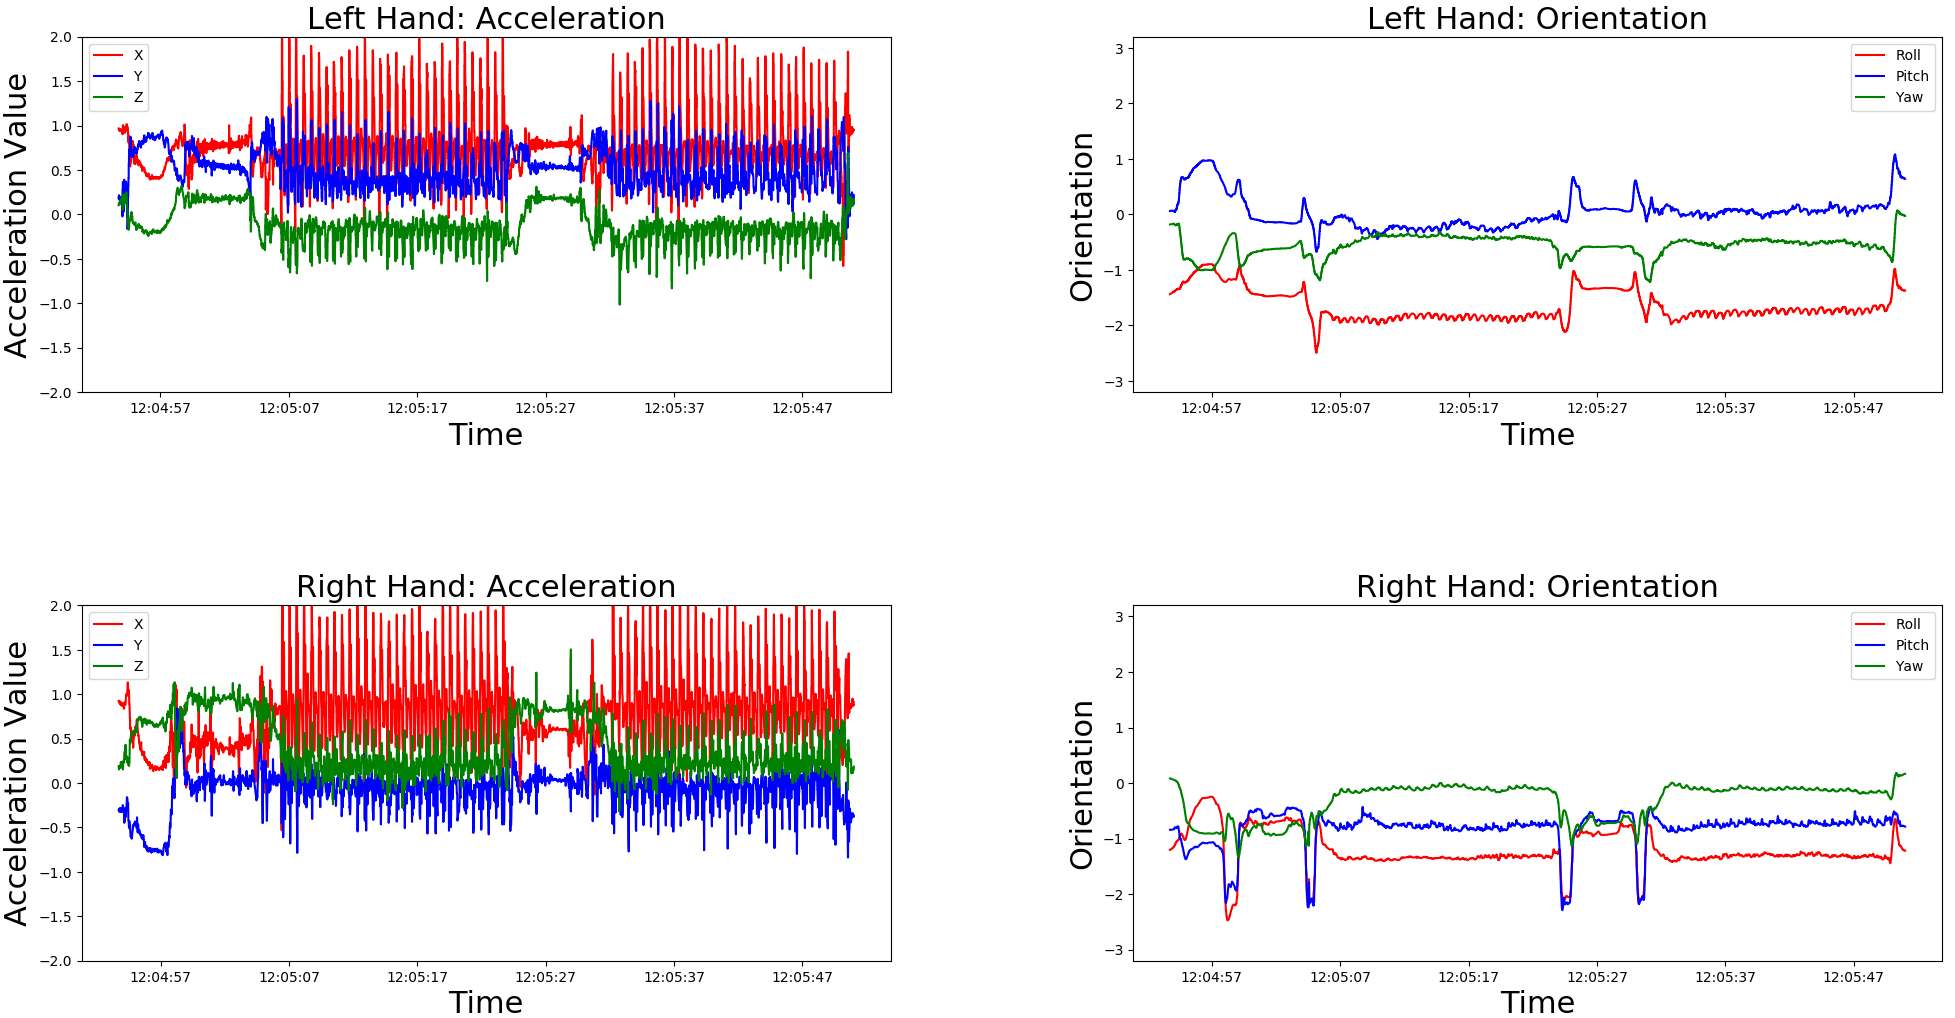
\includegraphics[width=\linewidth]{pictures/1571_IMU_Day3_cpr_31}
	\caption{IMU Data Plots for Acceleration and Orientation Data for CPR}
	\label{fig:1571imuday3cpr31}
\end{figure}
\begin{figure}[!h]
	\centering
	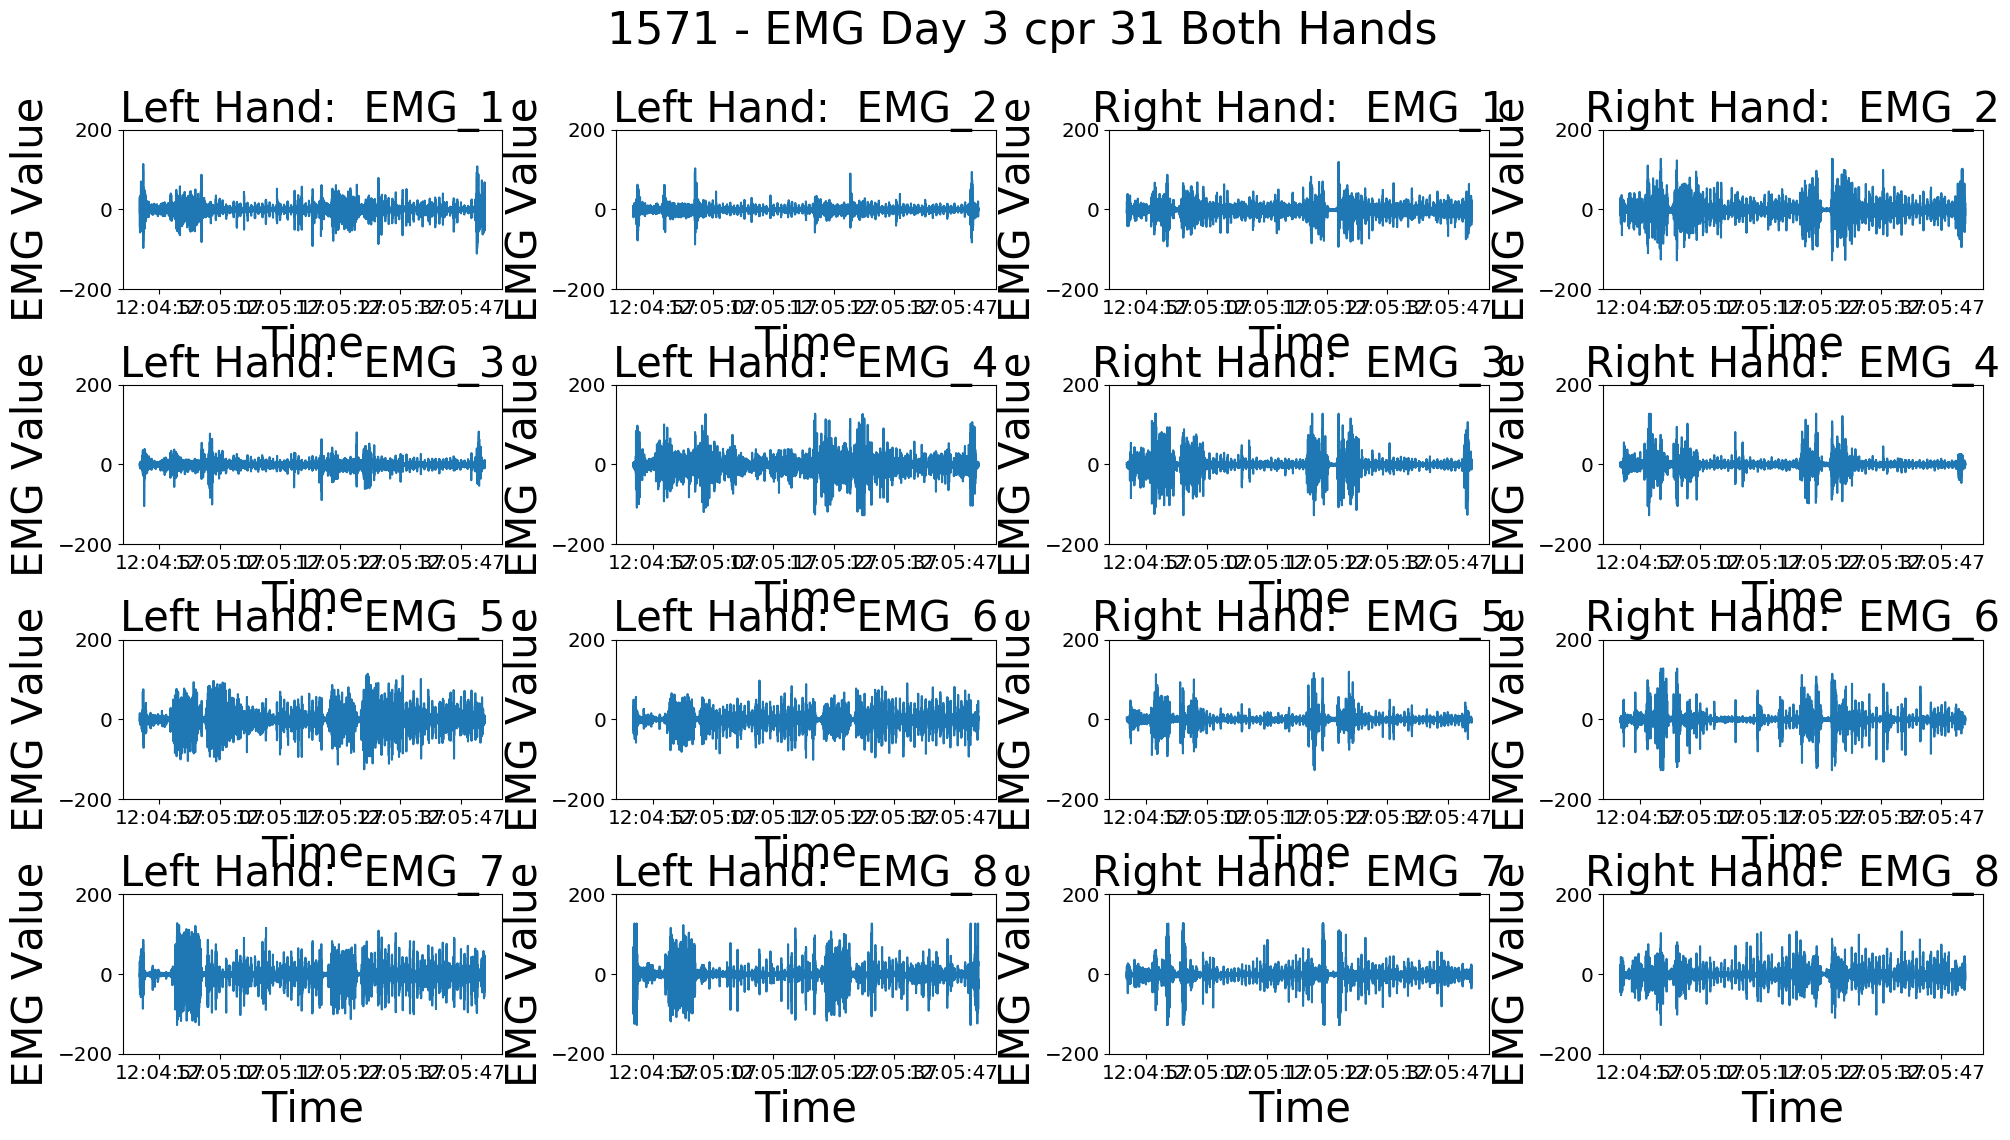
\includegraphics[width=\linewidth]{pictures/1571_EMG_Day3_cpr_31}
	\caption{EMG Data Plots for CPR}
	\label{fig:1571emgday3cpr31}
\end{figure}

Patients without adequate breathing are administered Bag-Valve-Mask ventilation. Completing one round of the Bag-Valve-Mask ventilation procedure took the participants an average of 35.39 seconds (St. Dev. = 5.70). The participants completed two rounds within one minute. The amount of instances for the third day were seven per participant, resulting in a total of 70 datasets.
\par The bag-valve-mask ventilation datasets consists of the unique squeezing the bag motion in the EMG sensor graph. The periodic motion is visible in all eight EMG channels in Figure \ref{fig:7073emgday3b46}. There was no prominent signal in the IMU data, as the right and left hands were stationary during this procedure. Figure \ref{fig:7073imuday3b46} shows almost flat lines for acceleration and orientation of both hands.
\begin{figure}[!h]
	\centering
	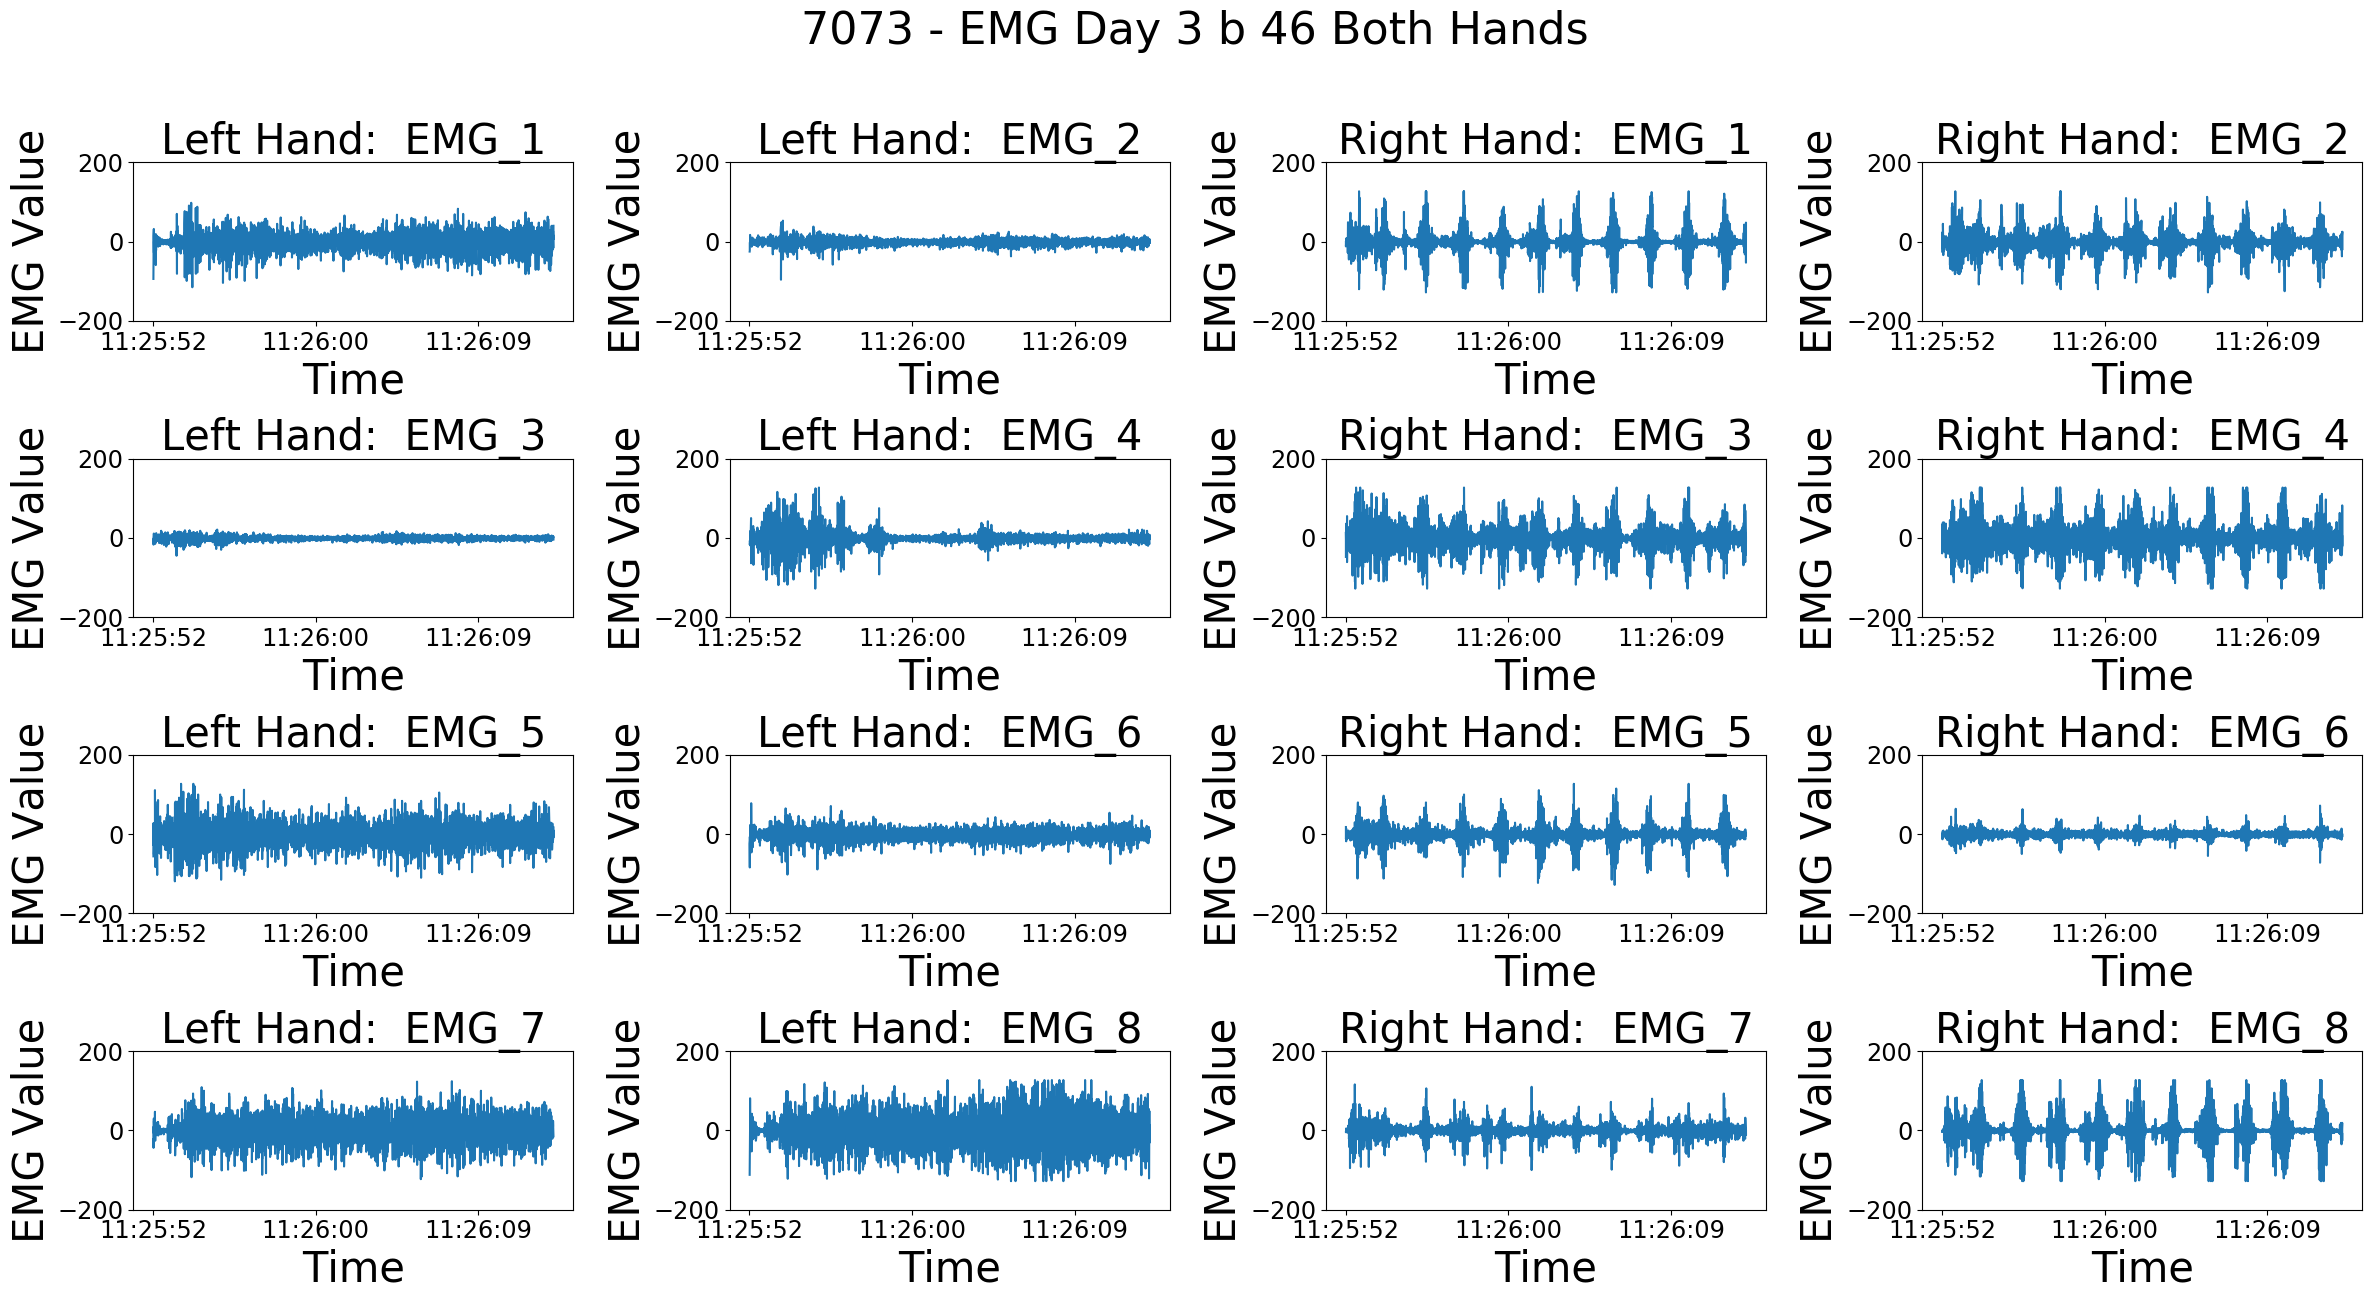
\includegraphics[width=\linewidth]{pictures/7073_EMG_Day3_b_46}
	\caption{EMG Data Plots for Bag-Valve-Mask ventilation}
	\label{fig:7073emgday3b46}
\end{figure}
\begin{figure}[!h]
	\centering
	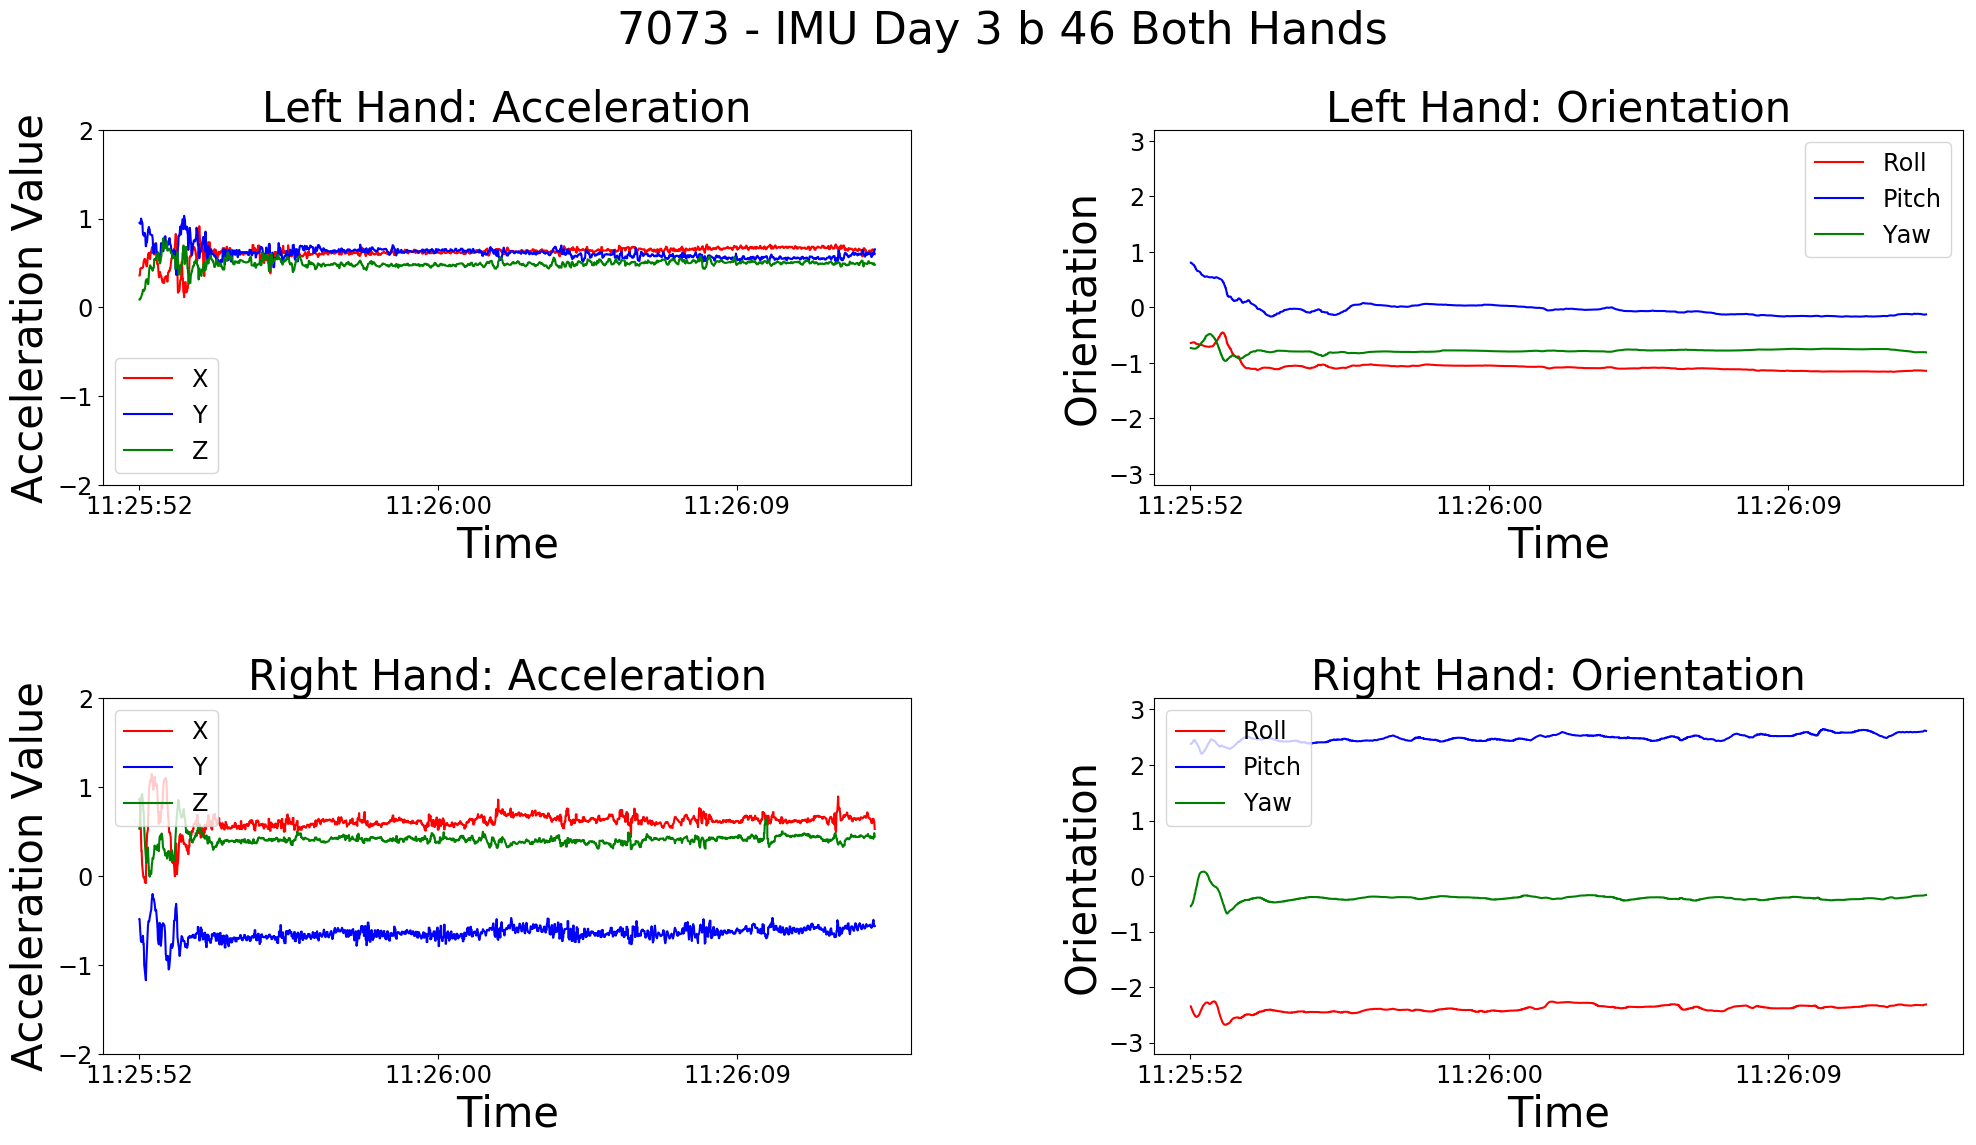
\includegraphics[width=\linewidth]{pictures/7073_IMU_Day3_b_46}
	\caption{IMU Data Plots for Acceleration and Orientation Data for Bag-Valve-Mask ventilation}
	\label{fig:7073imuday3b46}
\end{figure}

Placing an oral airway is part of the airway management procedures to prevent and relieve airway obstruction. The participants took an average of 6.51 seconds (St. Dev. = 2.23) to place an oral airway. The participants were able to complete an average of four rounds within one minute. The amount of instances for the third day were about 9 per participant, resulting in a total of about 90 instances.
\par Placing an oral airway requires the unique motion of rotating the oral airway 180 degrees after being inserted into the mouth. The rotating motion is visible in the right hand orientation graph starting at 15:14:32 with the bulge of the blue and red line in Figure \ref{fig:2334imuday3o22}. The acceleration data did not show any significant shapes of distribution. The EMG data in Figure \ref{fig:2334emgday3o22} shows a spike in channels three, four, and five when the oral airway is rotated.
\begin{figure}[!h]
	\centering
	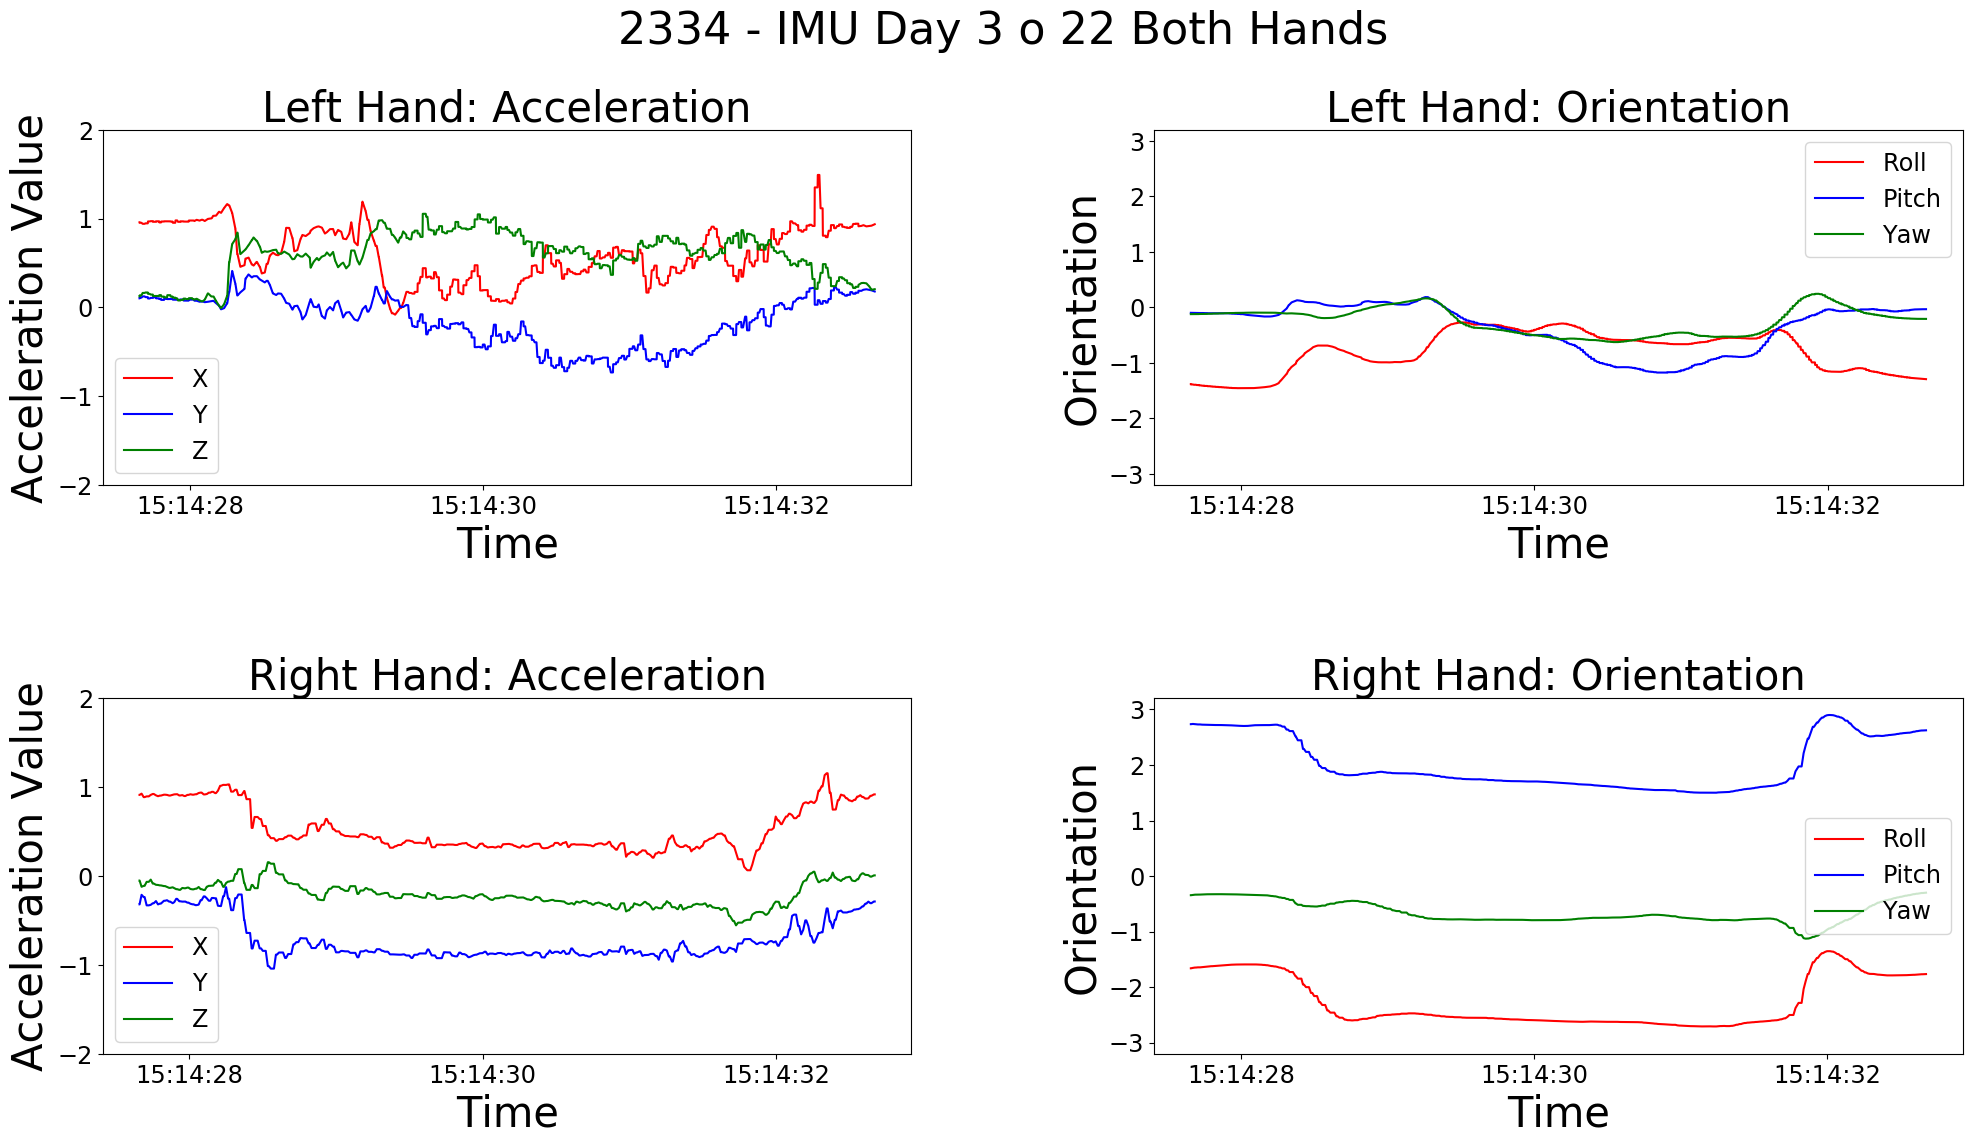
\includegraphics[width=\linewidth]{pictures/2334_IMU_Day3_o_22}
	\caption{IMU Data Plots for Acceleration and Orientation Data for Placing an Oral Airway}
	\label{fig:2334imuday3o22}
\end{figure}
\begin{figure}[!h]
	\centering
	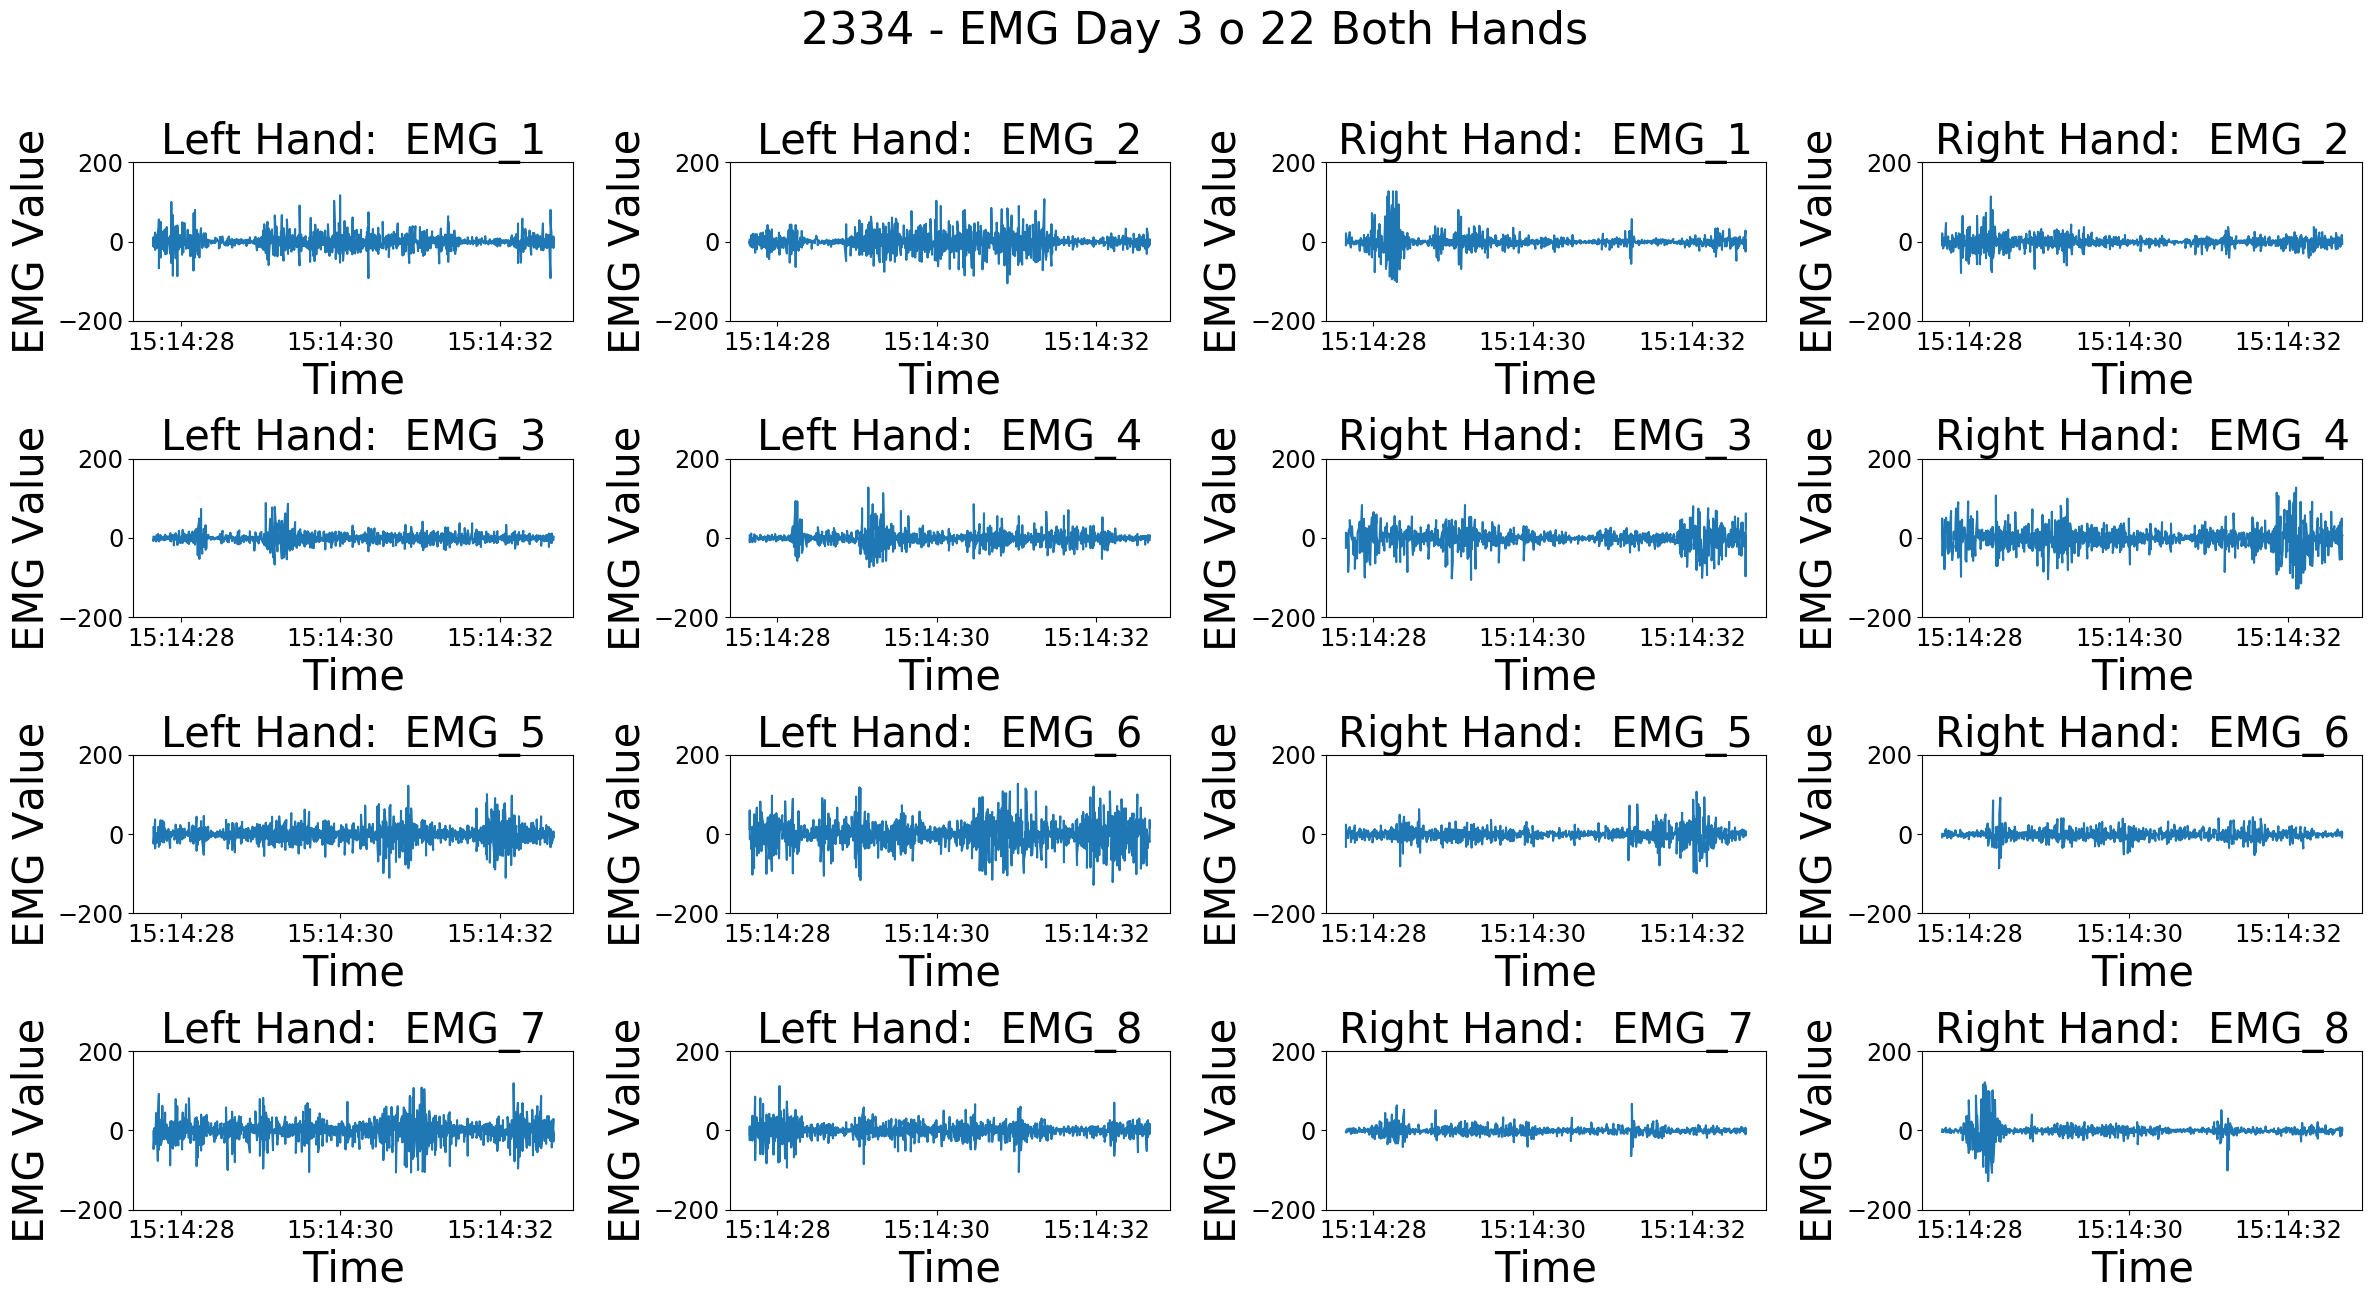
\includegraphics[width=\linewidth]{pictures/2334_EMG_Day3_o_22}
	\caption{EMG Data Plots for Placing an Oral Airway}
	\label{fig:2334emgday3o22}
\end{figure}

An intravenous tourniquet is used to restrict blood flow on a patient. The participants took an average of 9.38 seconds (St. Dev. = 2.70) to place an intravenous tourniquet. The participants were able to complete an average of three rounds within the one minute data collection of every procedure. The amount of instances for the third day were seven per participant, resulting in a total of 70 datasets.
\par The placing of an intravenous tourniquet consists of a single wrapping motion around the arm and tying of the ends. The wrapping and tying motion was visible in the IMU's orientation data starting at 9:09:09 with periodic movement and finishing at 09:09:15 with a spike in Figure \ref{fig:4501imuday3t7}. The acceleration and EMG in Figure \ref{fig:4501emgday3t7} data do not show any significant pattern.
\begin{figure}[!h]
	\centering
	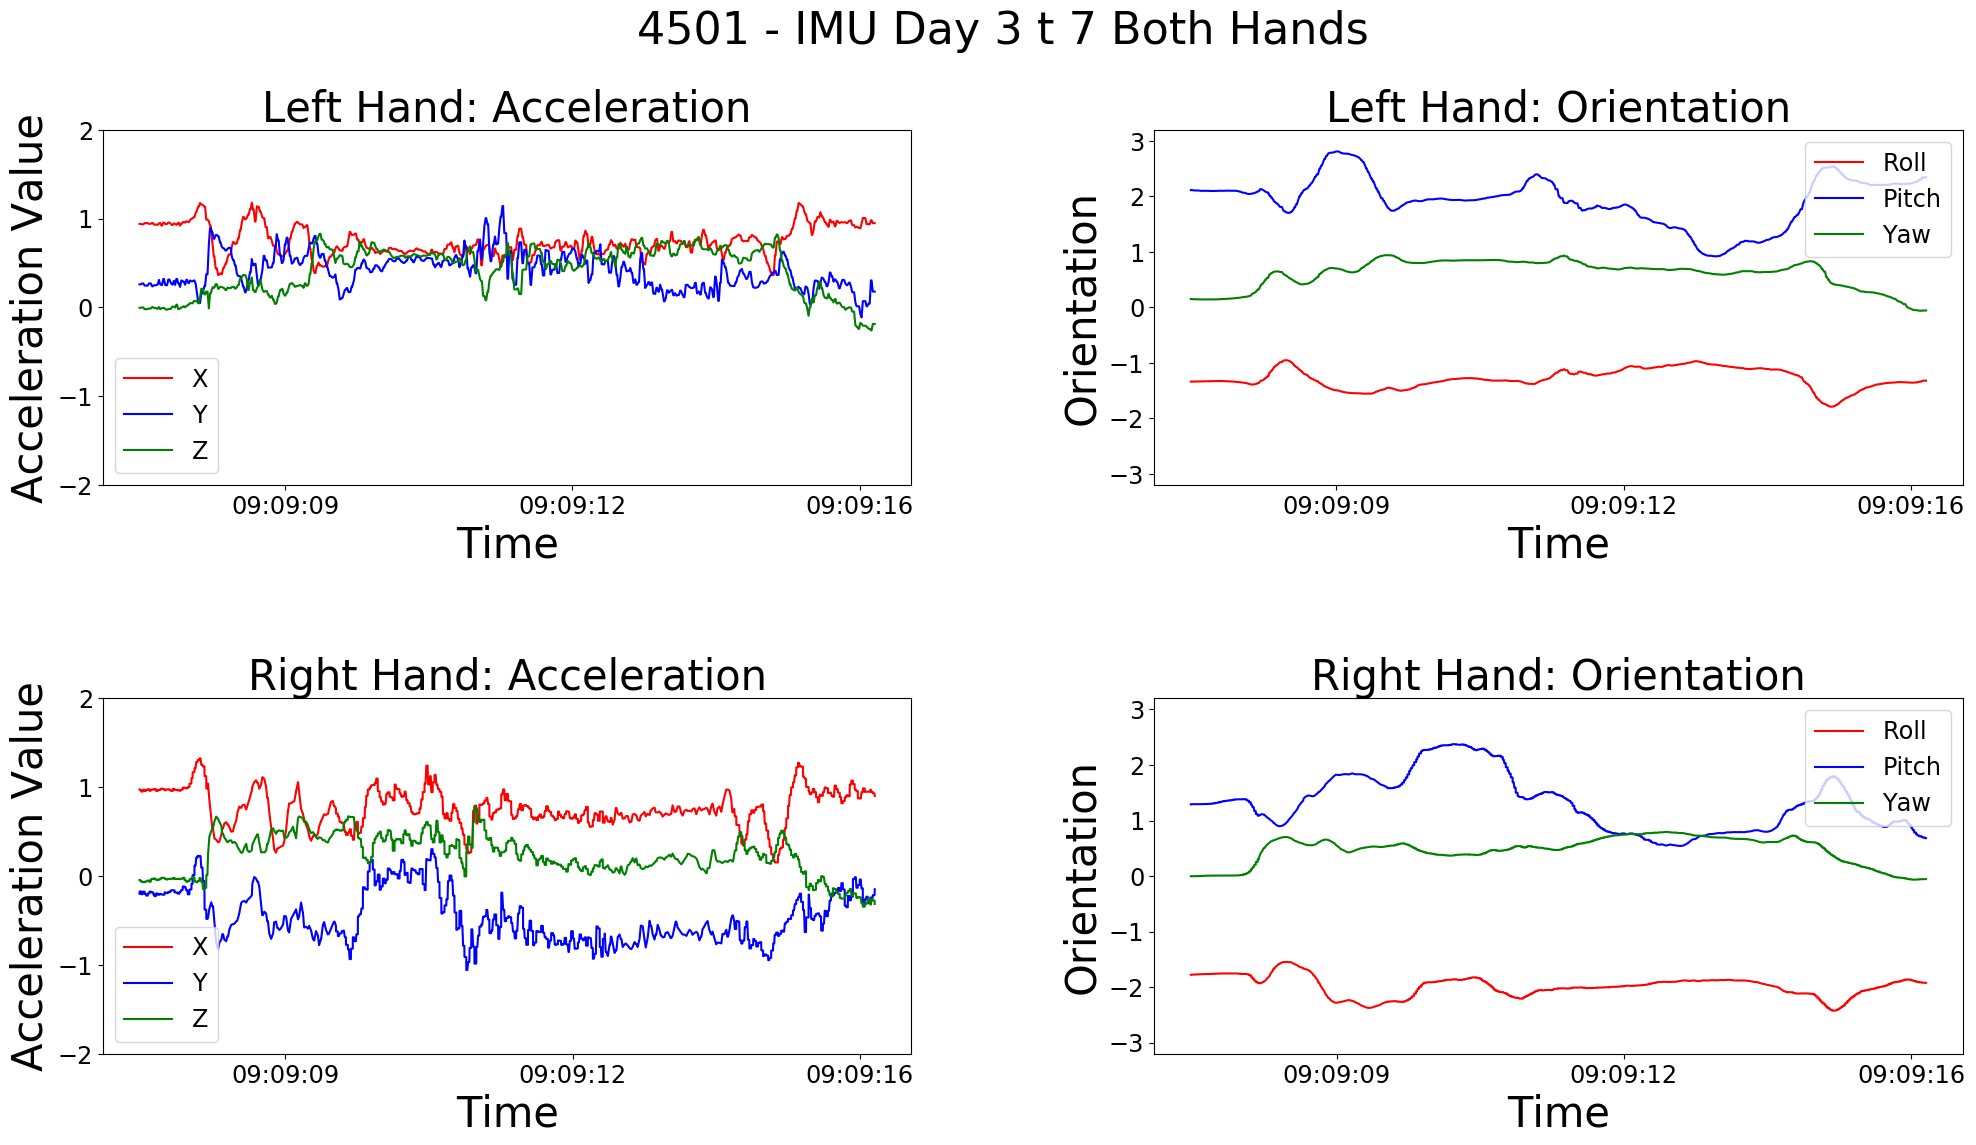
\includegraphics[width=\linewidth]{pictures/4501_IMU_Day3_t_7}
	\caption{IMU Data Plots for Acceleration and Orientation Data for Placing an IV Tourniquet}
	\label{fig:4501imuday3t7}
\end{figure}
\begin{figure}[!h]
	\centering
	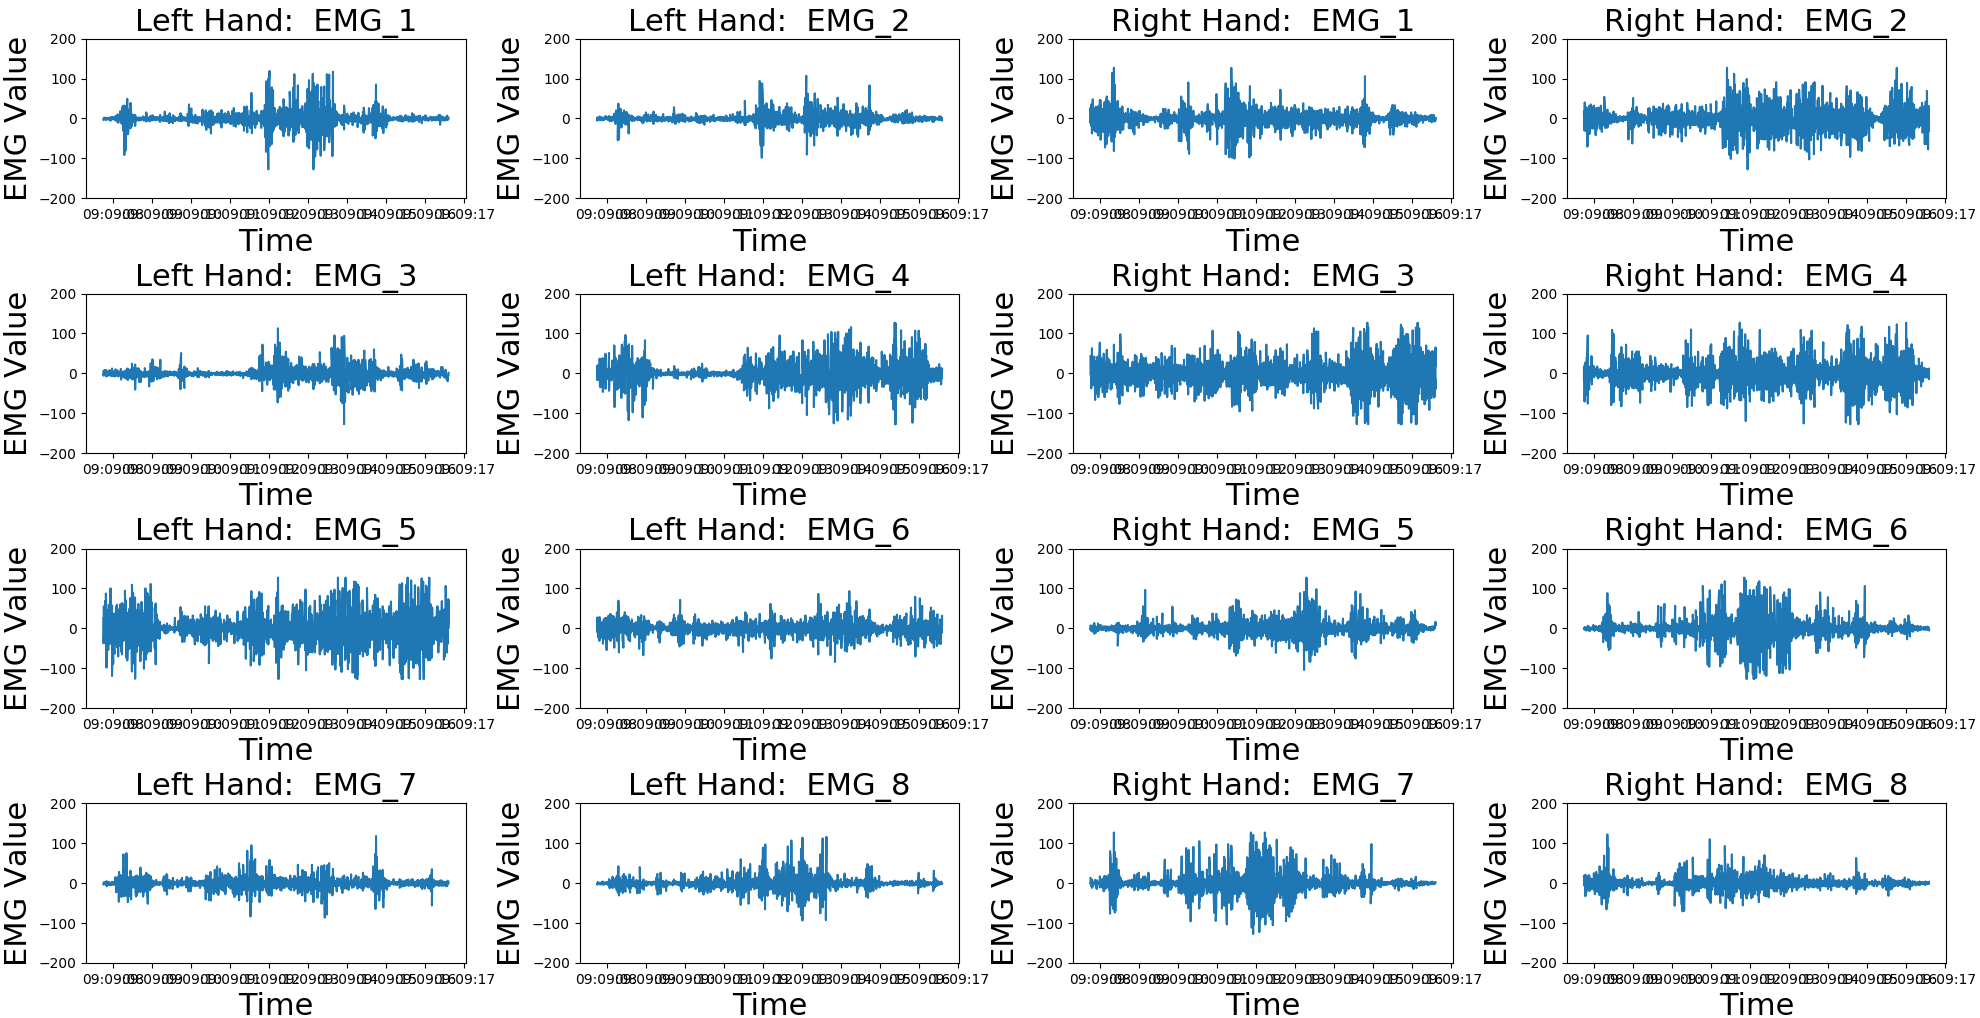
\includegraphics[width=\linewidth]{pictures/4501_EMG_Day3_t_7}
	\caption{EMG Data Plots for Placing an IV Tourniquet}
	\label{fig:4501emgday3t7}
\end{figure}

Wrapping a head wound is used to bandage a bleeding on a patient's head. Completely wrapping a head wound took participants an average of 37.26 seconds (St. Dev. = 11.72). The participants were able to complete two rounds within the one minute. The amount of instances for the third day were seven per participant, resulting in a total of 70 instances.
\par The Wrapping of a head wound consists of the unique movement of bandaging around the head of a patient. The wrapping motion is primarily visible in the orientation data of the IMU in Figure \ref{fig:2334imuday3w47}. The spikes in the orientation data at 15:27:18 are sinusoidal and represent the amount of rotations around the head. The EMG data in Figure \ref{fig:2334emgday3w47} shows a substantial amount of activity related to the grabbing and releasing of the bandage when wrapping around the patient's head.
\begin{figure}[!h]
	\centering
	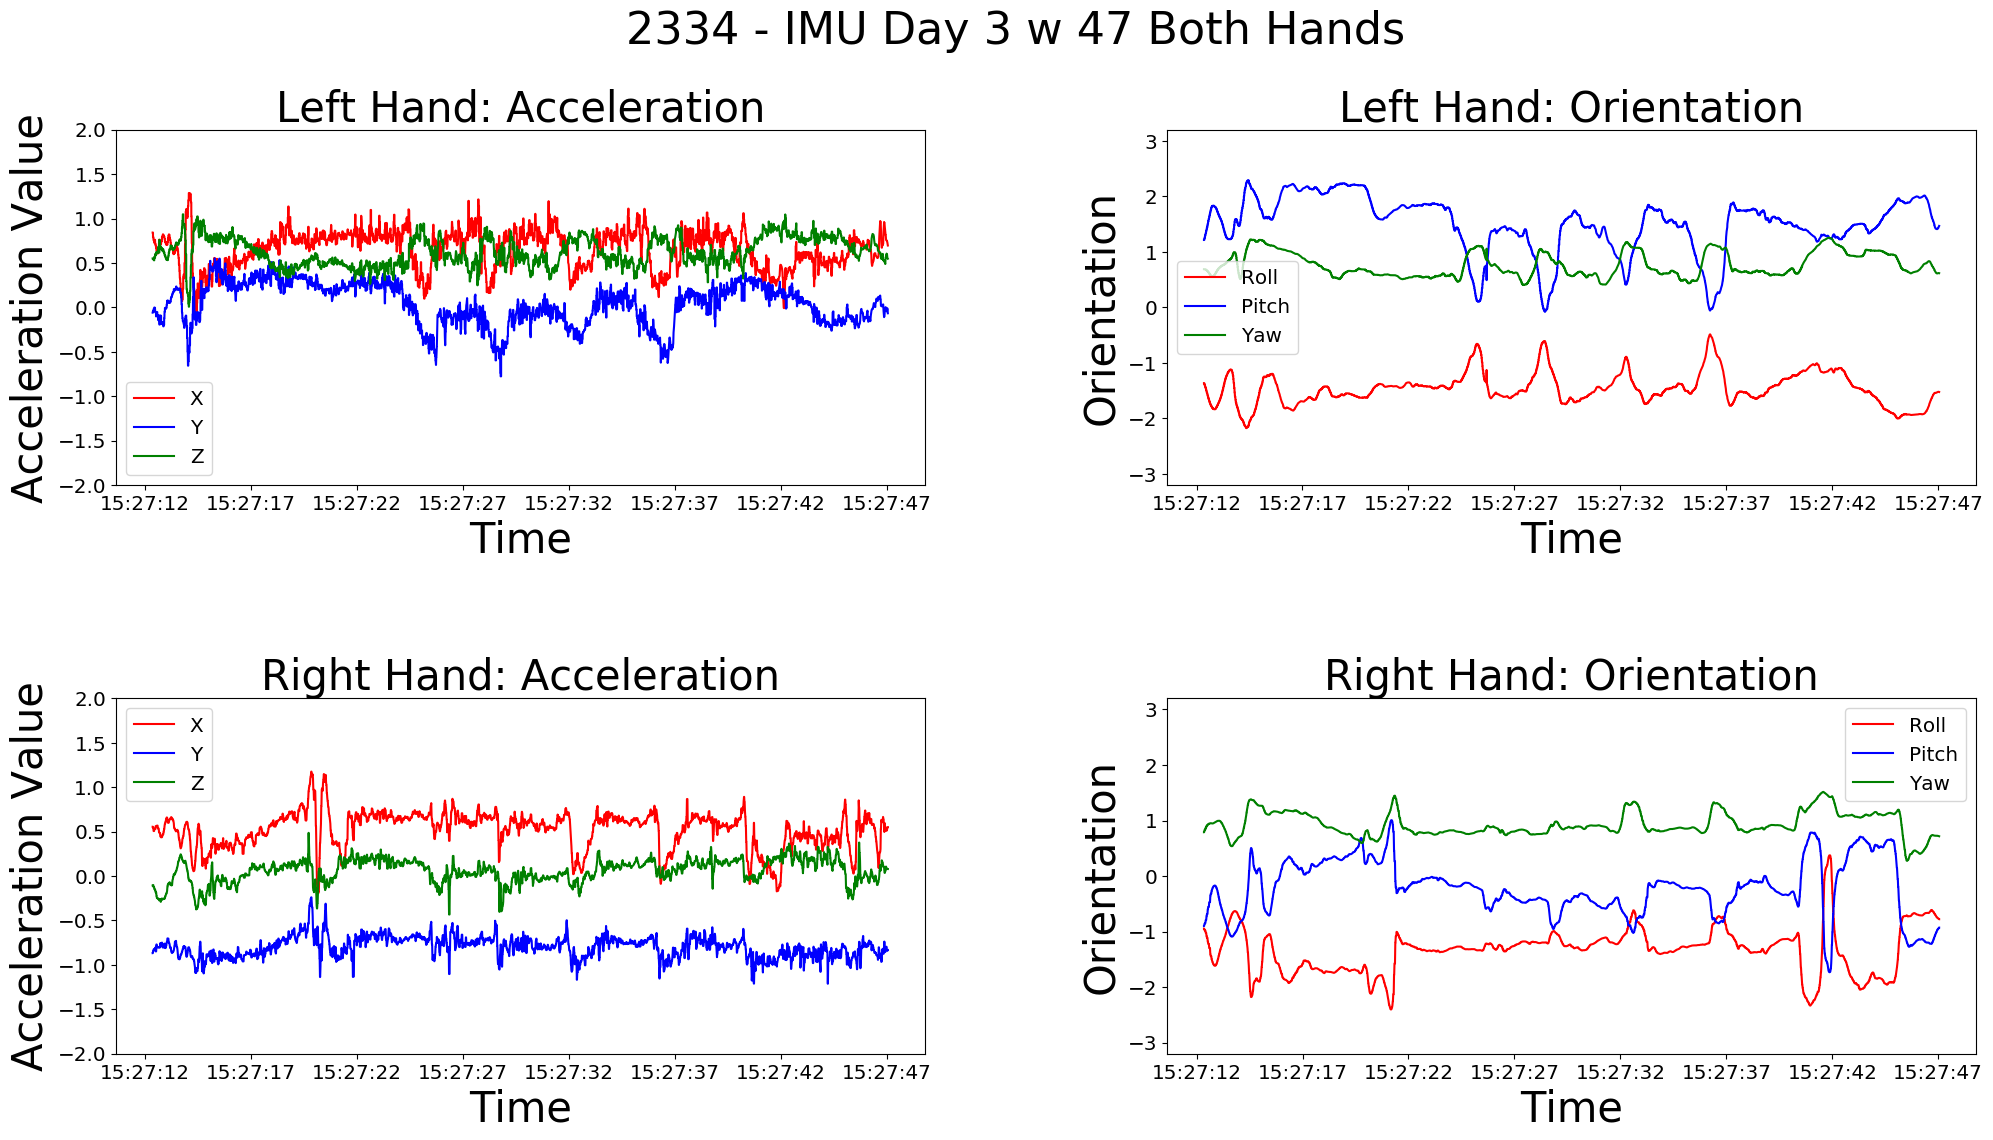
\includegraphics[width=\linewidth]{pictures/2334_IMU_Day3_w_47}
	\caption{IMU Data Plots for Acceleration and Orientation Data for wrapping a head wound}
	\label{fig:2334imuday3w47}
\end{figure}
\begin{figure}[!h]
	\centering
	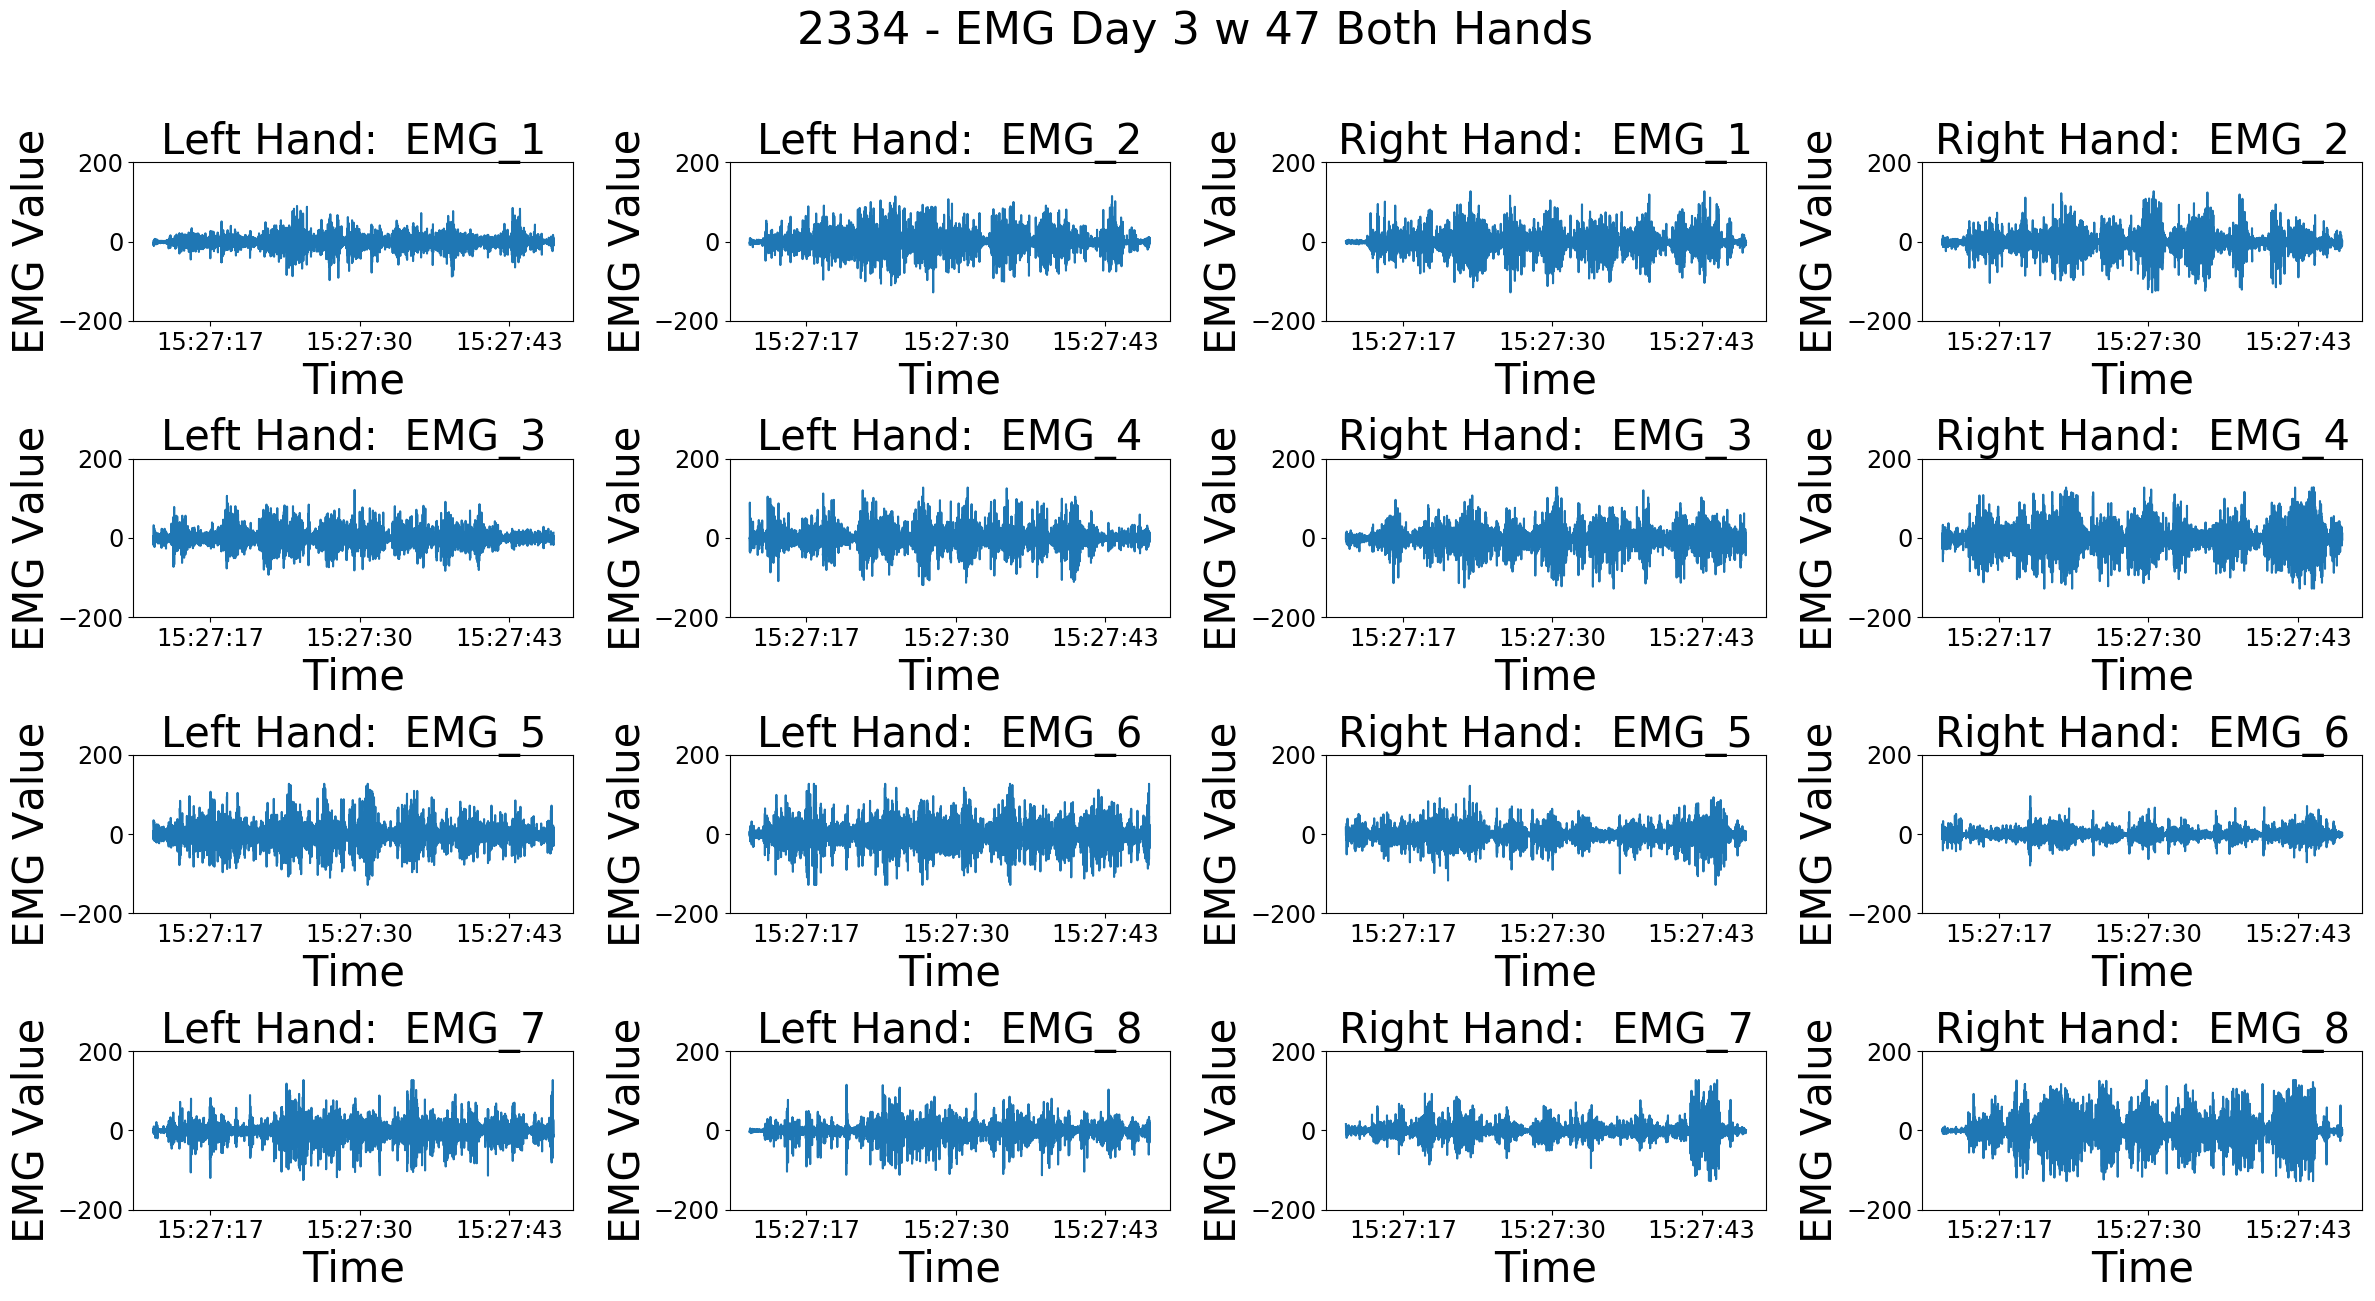
\includegraphics[width=\linewidth]{pictures/2334_EMG_Day3_w_47}
	\caption{EMG Data Plots for Wrapping a Head Wound}
	\label{fig:2334emgday3w47}
\end{figure}


\subsection{IMU and EMG Patterns Discussion}
\label{sec:Results:Patterns:Discussion}

\par The average time it takes to complete a procedure was used to detect potential outliers. Participants average time had to be within the standard deviation to be considered for the combined dataset of participant generalizability. Participant's 5 average time was outside of the overall average for all procedures and removed for the combined dataset.

\par The sinusoidal movement of the chest compressions in the acceleration data when performing the CPR procedure can make it easy for a machine learning algorithm to pick up on, due to the unique value for the signal magnitude area feature. The sequence of applying chest compressions twice during one run of the procedure can help the HMM algorithm identify CPR better, because of similar values occurring multiple times.

\par The Bag-Valve-Mask ventilation procedure has a unique movement repeatedly squeezing the bag. The repetitive motion will be clearly represented in the signal magnitude area feature as well as the standard deviation feature for the EMG data.

\par Placing a IV tourniquet and an oral airway took participants the shortest time to complete. These short procedures can make it harder for a machine learning algorithm to identify the procedure, as only few window iterations will occur during the length of the procedure.

\par The repeated wrapping motion of bandaging a head wound can help machine learning algorithm identify the procedure. The movement is clearly visible in both acceleration and orientation data of the IMU.

\par The patterns identified above can improve detection accuracy through the generated features when training machine learning algorithms with the collected data. The signal magnitude area is able to pick up periodic movement, the mean is able to generate a baseline of motion, and the standard deviation depicts the quantity of motion.


\section{Individual Participant Results}
\label{sec:Results:Individual}

Each individual participant's datasets were used to train the decision-tree, SVM, $k$-NN, and HMM machine learning algorithms. The F1, precision, and recall scores by participant for the CPR procedure are provided in Table \ref{tab:cpr:ml}. The first participant had the lowest F1 score of all machine learning algorithms with 0.69 for the decision-tree, 0.31 for $k$-NN, 0.28 for SVM, 0.00 for HMM. The HMM varied the most across participants when recognizing CPR .
\newcommand*\rotv{\multirow{2}{*}{\rotatebox[origin=c]{45}}}
\begin{table}[h]
	\centering
	\begin{tabular}{lllllllllllll}
		\multirow{2}{*}{\rotatebox[origin=c]{45}{\textbf{Participant}}} & \multicolumn{3}{c}{\textbf{decision-tree}} & \multicolumn{3}{c}{\textbf{$k$-NN} ($k=4$)} & \multicolumn{3}{c}{\textbf{SVM}} & \multicolumn{3}{c}{\textbf{HMM}} \\
		& \rot{Precision}     & \rot{Recall}    & \rot{F1}    & \rot{Precision}     & \rot{Recall}    & \rot{F1}  & \rot{Precision}     & \rot{Recall}    & \rot{F1} & \rot{Precision}     & \rot{Recall}    & \rot{F1} \\
		\textbf{1}   & \textbf{0.69} & \textbf{0.69} & \textbf{0.69} & 0.37 & 0.27 & 0.31 & 0.37 & 0.22 & 0.28 & 0.00 & 0.00 & 0.00 \\
		\textbf{2}   & \textbf{0.85} & 0.83 & 0.84 & 0.36 & 0.19 & 0.25 & 0.42 & 0.36 & 0.39 & 0.44 & 0.67 & 0.53 \\
		\textbf{3}   & \textbf{0.84} & 0.81 & 0.82 & 0.41 & 0.24 & 0.31 & 0.42 & 0.37 & 0.39 & 0.40 & 0.33 & 0.36 \\
		\textbf{4}   & 0.84 & \textbf{0.86} & 0.85 & 0.54 & 0.33 & 0.41 & 0.55 & 0.47 & 0.51 & 0.42 & 0.83 & 0.56 \\
		\textbf{5}   & 0.81 & \textbf{0.82} & \textbf{0.82} & 0.66 & 0.37 & 0.47 & 0.66 & 0.50 & 0.57 & 0.29 & 0.67 & 0.40 \\
		\textbf{6}   & 0.78 & \textbf{0.80} & 0.79 & 0.36 & 0.16 & 0.22 & 0.40 & 0.34 & 0.37 & 0.36 & 0.67 & 0.47 \\
		\textbf{7}   & 0.89 & \textbf{0.91} & 0.90 & 0.55 & 0.44 & 0.49 & 0.68 & 0.53 & 0.60 & 0.38 & 1.00 & 0.55 \\
		\textbf{8}   & 0.89 & \textbf{0.90} & 0.89 & 0.22 & 0.09 & 0.13 & 0.42 & 0.37 & 0.40 & 0.12 & 0.17 & 0.14 \\
		\textbf{9}   & \textbf{0.90} & 0.87 & 0.88 & 0.49 & 0.23 & 0.31 & 0.61 & 0.47 & 0.53 & 0.50 & 0.83 & 0.62 \\
		\textbf{10} & \textbf{0.83} & 0.77 & 0.80 & 0.50 & 0.27 & 0.35 & 0.54 & 0.45 & 0.49 & 0.50 & 0.67 & 0.57 \\
		\hline
		\textbf{Mean} & \textbf{0.83} & \textbf{0.83} & \textbf{0.83} & 0.45 & 0.26 & 0.33 & 0.51 & 0.41 & 0.45 & 0.34 & 0.58 & 0.42 \\
		\textbf{Std. Dev.} & 0.06 & 0.07 & 0.06 & 0.13 & 0.10 & 0.11 & 0.12 & 0.09 & 0.10 & 0.16 & 0.32 & 0.20
	\end{tabular}
	\caption{Ten-fold cross validation for detecting CPR per participant. Note: Bold represents the highest performance across a row}
	\label{tab:cpr:ml}
\end{table}

\par Bag-Valve-Mask ventilation achieved the lowest F1 scores of all procedures with F1 scores as low as 0.08 for participant eight using the $k$-NN algorithm, as seen in Table \ref{tab:bvm:ml}. The highest F1 score was achieved by participant ten using the HMM algorithm. The HMM algorithm also achieved the highest mean F1 score at 0.64 (Std. Dev=0.19), followed by the decision-tree algorithm at 0.60 (Std. Dev=0.09), and SVM algorithm at 0.26 (Std. Dev=0.06). The $k$-NN algorithm came last with a F1 score of 0.14 (Std. Dev=0.11).
\begin{table}[h]
	\centering
	\begin{tabular}{lllllllllllll}
		\multirow{2}{*}{\rotatebox[origin=c]{45}{\textbf{Participant}}}& \multicolumn{3}{c}{\textbf{decision-tree}} & \multicolumn{3}{c}{\textbf{$k$-NN} ($k=4$)} & \multicolumn{3}{c}{\textbf{SVM}} & \multicolumn{3}{c}{\textbf{HMM}} \\
		& \rot{Precision}     & \rot{Recall}    & \rot{F1}    & \rot{Precision}     & \rot{Recall}    & \rot{F1}  & \rot{Precision}     & \rot{Recall}    & \rot{F1} & \rot{Precision}     & \rot{Recall}    & \rot{F1} \\
		\textbf{1}   & \textbf{0.81} & 0.48 & 0.60 & 0.67 & 0.30 & 0.41 & 0.31 & 0.19 & 0.23 & 0.50 & 0.25 & 0.33 \\
		\textbf{2}   & 0.79 & 0.78 & 0.78 & 0.58 & 0.17 & 0.27 & 0.31 & 0.23 & 0.26 & 0.90 & 0.75 & \textbf{0.82} \\
		\textbf{3}   & 0.56 & 0.54 & 0.55 & 0.32 & 0.13 & 0.18 & 0.32 & 0.26 & 0.29 & \textbf{0.88} & 0.70 & 0.78 \\
		\textbf{4}   & 0.47 & 0.45 & 0.46 & 0.27 & 0.06 & 0.10 & 0.22 & 0.20 & 0.21 & \textbf{0.71} & 0.50 & 0.59 \\
		\textbf{5}   & 0.71 & 0.58 & 0.64 & 0.11 & 0.04 & 0.05 & 0.24 & 0.25 & 0.25 & \textbf{0.86} & 0.60 & 0.71 \\
		\textbf{6}   & \textbf{0.55} & 0.50 & 0.53 & 0.33 & 0.07 & 0.12 & 0.38 & 0.29 & 0.32 & 0.60 & 0.33 & 0.43 \\
		\textbf{7}   & 0.62 & 0.63 & 0.63 & 0.28 & 0.07 & 0.12 & 0.26 & 0.24 & 0.25 & \textbf{1.00} & 0.57 & 0.73 \\
		\textbf{8}   & 0.50 & \textbf{0.52} & 0.51 & 0.18 & 0.05 & 0.08 & 0.16 & 0.14 & 0.15 & 0.57 & 0.44 & 0.50 \\
		\textbf{9}   & \textbf{0.63} & 0.59 & 0.61 & 0.33 & 0.09 & 0.14 & 0.33 & 0.35 & 0.34 & 0.80 & 0.44 & 0.57 \\
		\textbf{10} & 0.67 & 0.63 & 0.65 & 0.12 & 0.02 & 0.03 & 0.30 & 0.33 & 0.32 & \textbf{1.00} & 0.90 & 0.95 \\
		\hline
		\textbf{Mean} & 0.63 & 0.57 & 0.60 & 0.31 & 0.10 & 0.14 & 0.28 & 0.25 & 0.26 & \textbf{0.78} & 0.55 & 0.64 \\
		\textbf{Std. Dev.} & 0.12 & 0.01 & 0.09 & 0.17 & 0.08 & 0.11 & 0.07 & 0.06 & 0.06 & 0.18 & 0.20 & 0.19
	\end{tabular}
	\caption{Ten-fold cross validation for detecting BVM ventilation per participant}
	\label{tab:bvm:ml}
\end{table}

\par Placing an oral airway was the most difficult procedure to detect, with F1 scores as low as 0.00 for participant five using $k$-NN, as seen in Table \ref{tab:o:ml}. The highest F1 score was achieved by participant four using the HMM algorithm. The decision-tree classifier was the algorithm with the highest mean F1 score at 0.63 (Std. Dev=0.08), followed by the HMM algorithm at 0.51 (Std. Dev=0.27), and SVM algorithm at 0.20 (Std. Dev=0.04). The $k$-NN algorithm came last with a F1 score of 0.12 (Std. Dev=0.08).
\begin{table}[h]
	\centering
	\begin{tabular}{lllllllllllll}
		\multirow{2}{*}{\rotatebox[origin=c]{45}{\textbf{Participant}}} & \multicolumn{3}{c}{\textbf{decision-tree}} & \multicolumn{3}{c}{\textbf{$k$-NN} ($k=4$)} & \multicolumn{3}{c}{\textbf{SVM}} & \multicolumn{3}{c}{\textbf{HMM}} \\
		& \rot{Precision}     & \rot{Recall}    & \rot{F1}    & \rot{Precision}     & \rot{Recall}    & \rot{F1}  & \rot{Precision}     & \rot{Recall}    & \rot{F1} & \rot{Precision}     & \rot{Recall}    & \rot{F1} \\
		\textbf{1}   & 0.47 & \textbf{0.58} & 0.52 & 0.26 & 0.14 & 0.18 & 0.24 & 0.18 & 0.21 & 0.00 & 0.00 & 0.00 \\
		\textbf{2}   & 0.63 & 0.56 & 0.59 & 0.29 & 0.10 & 0.15 & 0.19 & 0.21 & 0.20 & \textbf{1.00} & 0.50 & 0.67 \\
		\textbf{3}   & 0.67 & 0.76 & 0.71 & 0.50 & 0.17 & 0.25 & 0.29 & 0.24 & 0.26 & \textbf{0.78} & 0.70 & 0.74 \\
		\textbf{4}   & 0.68 & 0.65 & 0.66 & 0.44 & 0.10 & 0.17 & 0.26 & 0.21 & 0.23 & \textbf{0.86} & 0.67 & 0.75 \\
		\textbf{5}   & \textbf{0.66} & \textbf{0.66} & \textbf{0.66} & 0.00 & 0.00 & 0.00 & 0.29 & 0.17 & 0.22 & 0.62 & 0.56 & 0.59 \\
		\textbf{6}   & 0.71 & 0.71 & 0.71 & 0.27 & 0.06 & 0.10 & 0.16 & 0.15 & 0.16 & \textbf{0.75} & 0.67 & 0.71 \\
		\textbf{7}   & \textbf{0.60} & 0.59 & \textbf{0.60} & 0.12 & 0.03 & 0.05 & 0.23 & 0.18 & 0.20 & 0.50 & 0.14 & 0.22 \\
		\textbf{8}   & 0.71 & \textbf{0.78} & 0.74 & 0.38 & 0.12 & 0.19 & 0.28 & 0.20 & 0.23 & 0.25 & 0.11 & 0.15 \\
		\textbf{9}   & 0.62 & 0.66 & 0.64 & 0.09 & 0.04 & 0.05 & 0.15 & 0.11 & 0.13 & \textbf{0.80} & 0.50 & 0.62 \\
		\textbf{10} & 0.54 & 0.59 & 0.57 & 0.40 & 0.06 & 0.10 & 0.16 & 0.13 & 0.14 & \textbf{0.67} & 0.57 & 0.62 \\
		\hline
		\textbf{Mean} & 0.63 & \textbf{0.65} & 0.63 & 0.28 & 0.08 & 0.12 & 0.22 & 0.18 & 0.20 & 0.62 & 0.44 & 0.51 \\
		\textbf{Std. Dev.} & 0.08 & 0.08 & 0.08 & 0.16 & 0.05 & 0.08 & 0.06 & 0.04 & 0.04 & 0.30 & 0.26 & 0.27 \\
	\end{tabular}
	\caption{Ten-fold cross validation for detecting oral airway placement per participant}
	\label{tab:o:ml}
\end{table}

\par Placing an IV tourniquet achieved a good F1 score for all machine learning algorithms except the HMM algorithm, as seen in Table \ref{tab:t:ml}. The lowest F1 score of 0.00 were achieved by participants two, three, and five. The highest F1 score was 0.87 by participant eight using the decision-tree. The decision-tree classifier was the algorithm with the highest mean F1 score at 0.81 (Std. Dev=0.06), followed by the SVM algorithm at 0.53 (Std. Dev=0.10), and $k$-NN at 0.40 (Std. Dev=0.05). The HMM algorithm came last with a F1 score of 0.24 (Std. Dev=0.21).
\begin{table}[h]
	\centering
	\begin{tabular}{lllllllllllll}
		\multirow{2}{*}{\rotatebox[origin=c]{45}{\textbf{Participant}}} & \multicolumn{3}{c}{\textbf{decision-tree}} & \multicolumn{3}{c}{\textbf{$k$-NN} ($k=4$)} & \multicolumn{3}{c}{\textbf{SVM}} & \multicolumn{3}{c}{\textbf{HMM}} \\
		& \rot{Precision}     & \rot{Recall}    & \rot{F1}    & \rot{Precision}     & \rot{Recall}    & \rot{F1}  & \rot{Precision}     & \rot{Recall}    & \rot{F1} & \rot{Precision}     & \rot{Recall}    & \rot{F1} \\
		\textbf{1}   & \textbf{0.65} & \textbf{0.65} & \textbf{0.65} & 0.30 & 0.36 & 0.33 & 0.29 & 0.30 & 0.30 & 0.22 & 0.40 & 0.29 \\
		\textbf{2}   & 0.80 & \textbf{0.81} & 0.80 & 0.31 & 0.56 & 0.40 & 0.51 & 0.62 & 0.56 & 0.00 & 0.00 & 0.00 \\
		\textbf{3}   & \textbf{0.83} & 0.81 & 0.82 & 0.30 & 0.57 & 0.39 & 0.43 & 0.56 & 0.49 & 0.00 & 0.00 & 0.00 \\
		\textbf{4}   & 0.84 & \textbf{0.85} & 0.84 & 0.37 & 0.64 & 0.47 & 0.56 & 0.67 & 0.61 & 0.50 & 0.17 & 0.25 \\
		\textbf{5}   & 0.85 & \textbf{0.87} & 0.86 & 0.34 & 0.64 & 0.45 & 0.54 & 0.71 & 0.61 & 0.00 & 0.00 & 0.00 \\
		\textbf{6}   & \textbf{0.83} & 0.80 & 0.82 & 0.31 & 0.42 & 0.36 & 0.48 & 0.59 & 0.53 & 0.33 & 0.17 & 0.22 \\
		\textbf{7}   & \textbf{0.80} & 0.79 & \textbf{0.80} & 0.27 & 0.44 & 0.33 & 0.42 & 0.55 & 0.48 & 0.22 & 0.33 & 0.27 \\
		\textbf{8}   & \textbf{0.89} & 0.86 & 0.87 & 0.33 & 0.60 & 0.43 & 0.50 & 0.66 & 0.57 & 0.60 & 0.50 & 0.55 \\
		\textbf{9}   & \textbf{0.80} & 0.78 & 0.79 & 0.34 & 0.53 & 0.41 & 0.47 & 0.59 & 0.53 & 0.75 & 0.50 & 0.60 \\
		\textbf{10} & 0.80 & \textbf{0.84} & 0.82 & 0.28 & 0.52 & 0.37 & 0.43 & 0.53 & 0.58 & 0.25 & 0.17 & 0.20 \\
		\hline
		\textbf{Mean} & \textbf{0.81} & \textbf{0.81} & \textbf{0.81} & 0.32 & 0.52 & 0.40 & 0.46 & 0.60 & 0.53 & 0.30 & 0.22 & 0.24 \\
		\textbf{Std. Dev.} & 0.06 & 0.06 & 0.06 & 0.03 & 0.10 & 0.05 & 0.08 & 0.11 & 0.10 & 0.26 & 0.20 & 0.21
	\end{tabular}
	\caption{Ten-fold cross validation for detecting tourniquet placement per participant}
	\label{tab:t:ml}
\end{table}

\par Wrapping a head wound achieved the highest F1 for the decision-tree algorithm of 0.93 for participants eight and ten, as seen in Table \ref{tab:w:ml}. The lowest F1 score was 0.00 for participant seven using the HMM algorithm. The decision-tree classifier had a mean F1 score of 0.90 (Std. Dev=0.06), followed by the SVM algorithm at 0.61 (Std. Dev=0.04), and $k$-NN at 0.50 (Std. Dev=0.04). The HMM algorithm came last with a F1 score of 0.40 (Std. Dev=0.18)
\begin{table}[]
	\centering
	\begin{tabular}{lllllllllllll}
		\multirow{2}{*}{\rotatebox[origin=c]{45}{\textbf{Participant}}} & \multicolumn{3}{c}{\textbf{decision-tree}} & \multicolumn{3}{c}{\textbf{$k$-NN} ($k=4$)} & \multicolumn{3}{c}{\textbf{SVM}} & \multicolumn{3}{c}{\textbf{HMM}} \\
		& \rot{Precision}     & \rot{Recall}    & \rot{F1}    & \rot{Precision}     & \rot{Recall}    & \rot{F1}  & \rot{Precision}     & \rot{Recall}    & \rot{F1} & \rot{Precision}     & \rot{Recall}    & \rot{F1} \\
		\textbf{1}   & \textbf{0.73} & 0.72 & 0.72 & 0.43 & 0.54 & 0.48 & 0.47 & 0.66 & 0.55 & 0.20 & 0.20 & 0.20 \\
		\textbf{2}   & 0.88 & \textbf{0.91} & 0.89 & 0.45 & 0.46 & 0.46 & 0.60 & 0.58 & 0.59 & 0.30 & 0.50 & 0.37 \\
		\textbf{3}   & 0.81 & \textbf{0.83} & 0.82 & 0.42 & 0.42 & 0.42 & 0.63 & 0.62 & 0.62 & 0.38 & 0.83 & 0.53 \\
		\textbf{4}   & \textbf{0.91} & 0.90 & 0.90 & 0.43 & 0.49 & 0.46 & 0.61 & 0.63 & 0.62 & 0.22 & 0.33 & 0.27 \\
		\textbf{5}   & \textbf{0.87} & \textbf{0.87} & \textbf{0.87} & 0.42 & 0.39 & 0.40 & 0.63 & 0.63 & 0.63 & 0.29 & 0.33 & 0.31 \\
		\textbf{6}   & 0.88 & \textbf{0.90} & 0.89 & 0.45 & 0.65 & 0.53 & 0.54 & 0.55 & 0.55 & 0.44 & 0.67 & 0.53 \\
		\textbf{7}   & \textbf{0.92} & 0.91 & \textbf{0.92} & 0.49 & 0.54 & 0.51 & 0.60 & 0.65 & 0.62 & 0.00 & 0.00 & 0.00 \\
		\textbf{8}   & \textbf{0.94} & 0.92 & 0.93 & 0.43 & 0.48 & 0.45 & 0.62 & 0.59 & 0.61 & 0.25 & 0.50 & 0.33 \\
		\textbf{9}   & 0.88 & \textbf{0.90} & 0.89 & 0.49 & 0.55 & 0.51 & 0.68 & 0.68 & 0.68 & 0.45 & 0.83 & 0.59 \\
		\textbf{10} & 0.92 & \textbf{0.93} & \textbf{0.93} & 0.44 & 0.51 & 0.47 & 0.66 & 0.67 & 0.67 & 0.38 & 0.50 & 0.43 \\
		\hline
		\textbf{Mean} & \textbf{0.90} & \textbf{0.90} & \textbf{0.90} & 0.44 & 0.50 & 0.50 & 0.60 & 0.63 & 0.61 & 0.30 & 0.50 & 0.40 \\
		\textbf{Std. Dev.} & 0.06 & 0.06 & 0.06 & 0.03 & 0.07 & 0.04 & 0.06 & 0.04 & 0.04 & 0.13 & 0.30 & 0.18
	\end{tabular}
	\caption{Ten-fold cross validation for detecting wrapping a wound per participant}
	\label{tab:w:ml}
\end{table}

\subsection{Individual Participant Results Discussion}
\label{sec:Results:Individual:Discussion}
Contrary to the initial assumption in $H_1$, recognition of CPR and Bag-valve-mask ventilation will have the highest accuracy for each machine learning algorithm, due to its unique movements, the unique movements during CPR were not as helpful to accurately detect the procedure. The hypothesis was not supported. The overlap of the giving breaths motion resulted in CPR being misclassified as Bag-Valve-Mask ventilation. Segmenting out the chest-compressions from the breathing motions and only training using the chest-compressions may result in higher accuracy due to the chest-compressions not appearing in any other procedure.
\par Results between the participants varied greatly. The HMM algorithm scored 0.61 for one participant and 0.00 for another participant, see Table \ref{tab:cpr:ml}. Other algorithms, such as decision-tree and SVM were more stable as indicated by a low standard deviation.
\par The Bag-Valve-Mask ventilation procedure has such a unique squeezing movement that the initial assumption concluded that it will be one of the easiest procedures to detect. In contrast it turned out to be one of the hardest, which may be due to its movement overlap with CPR.
\par The F1 scores show that detecting the placement of an oral airway is challenging. The short duration for the placemet does not leave much time for the algorithm to detect unique movements. The grabbing and spinning motion can occur in several other procedures when equipment are picked up and put into place.
\par The low score of the HMM algorithm for placing an intravenous tourniquet can be a result of a close log probability of the HMM models. The HMM algorithm picks the highest log probability when data is tested on all HMM models. If the log probability are close it can mean the motion is easily interchangeable.
\par The HMM algorithm for wrapping a head wound under performed at detecting the procedure and had the highest standard deviation across participants. Participant seven achieved 0.92 for the decision-tree algorithm, but 0.00 for the HMM algorithm. The wide gap between recognition scores can contribute to the problem the HMM algorithm has with selecting the best model given the log probabilities.

\section{Participant Generalizability}
\label{sec:Results:Generalizability}

The datasets of all participants is combined to create one large dataset. The F1 score in Table \ref{tab:ml} is lower when comparing the machine learning algorithms on the combined dataset to the individual participants, Tables \ref{tab:cpr:ml} through \ref{tab:w:ml}. The highest F1 score on the combined dataset is achieved by the decision-tree algorithm with 0.71. The HMM algorithm followed second with 0.44, then $k$-NN with 0.35, and last the SVM with 0.25. Wrapping a wound (W) was the procedure with the highest F1 score for the decision-tree, $k$-NN ($k=4$) and SVM algorithm. Bag-Valve-Mask ventilation (B) was the procedure with the highest F1 score for the HMM algorithm.
\begin{table}[!h]
	\centering
	\begin{tabular}{lllllllllllll}
		\multirow{2}{*}{\rotatebox[origin=c]{45}{\textbf{Procedure}}} & \multicolumn{3}{c}{\textbf{decision-tree}} & \multicolumn{3}{c}{\textbf{$k$-NN} ($k=4$)} & \multicolumn{3}{c}{\textbf{SVM}} & \multicolumn{3}{c}{\textbf{HMM}} \\
		 & \rot{Precision}     & \rot{Recall}    & \rot{F1}    & \rot{Precision}     & \rot{Recall}    & \rot{F1}  & \rot{Precision}     & \rot{Recall}    & \rot{F1} & \rot{Precision}     & \rot{Recall}    & \rot{F1} \\
		 T & 0.73 & 0.74 & 0.74 & 0.33 & 0.56 & 0.41 & 0.53 & 0.62 & 0.57 & 0.29 & 0.36 & 0.32 \\
		 W & 0.82 & 0.82 & 0.82 & 0.42 & 0.45 & 0.43 & 0.57 & 0.72 & 0.64 & 0.19 & 0.20 & 0.20 \\
		 B & 0.39 & 0.38 & 0.39 & 0.24 & 0.07 & 0.11 & 0.18 & 0.10 & 0.13 & 0.69 & 0.71 & 0.70 \\
		 O & 0.48 & 0.46 & 0.47 & 0.23 & 0.06 & 0.10 & 0.25 & 0.13 & 0.17 & 0.60 & 0.33 & 0.43 \\
		 C & 0.69 & 0.69 & 0.69 & 0.42 & 0.27 & 0.33 & 0.48 & 0.35 & 0.41 & 0.39 & 0.50 & 0.44 \\
		 \hline
		 All & 0.71 & 0.71 & 0.71 & 0.37 & 0.37 & 0.35 & 0.49 & 0.52 & 0.49 & 0.47 & 0.44 & 0.44 \\
	\end{tabular}
	\caption{Ten-fold cross validation for all participants by procedure and algorithm. Note: T is intravenous tourniquet, W is wrapping a wound, B is Bag-Valve-Mask ventilation, O is oral airway, and C is CPR}
	\label{tab:ml}
\end{table}
The differences in movement between participants can be seen in Figure \ref{fig:5187emgday3t1average}. The Figure shows the average of placing an intravenous tourniquet for all participants in red. Similarities between the average EMG data and the data of the participant can be seen, yet some noise is observable in channels three, four, and five.
\begin{figure}[!h]
	\centering
	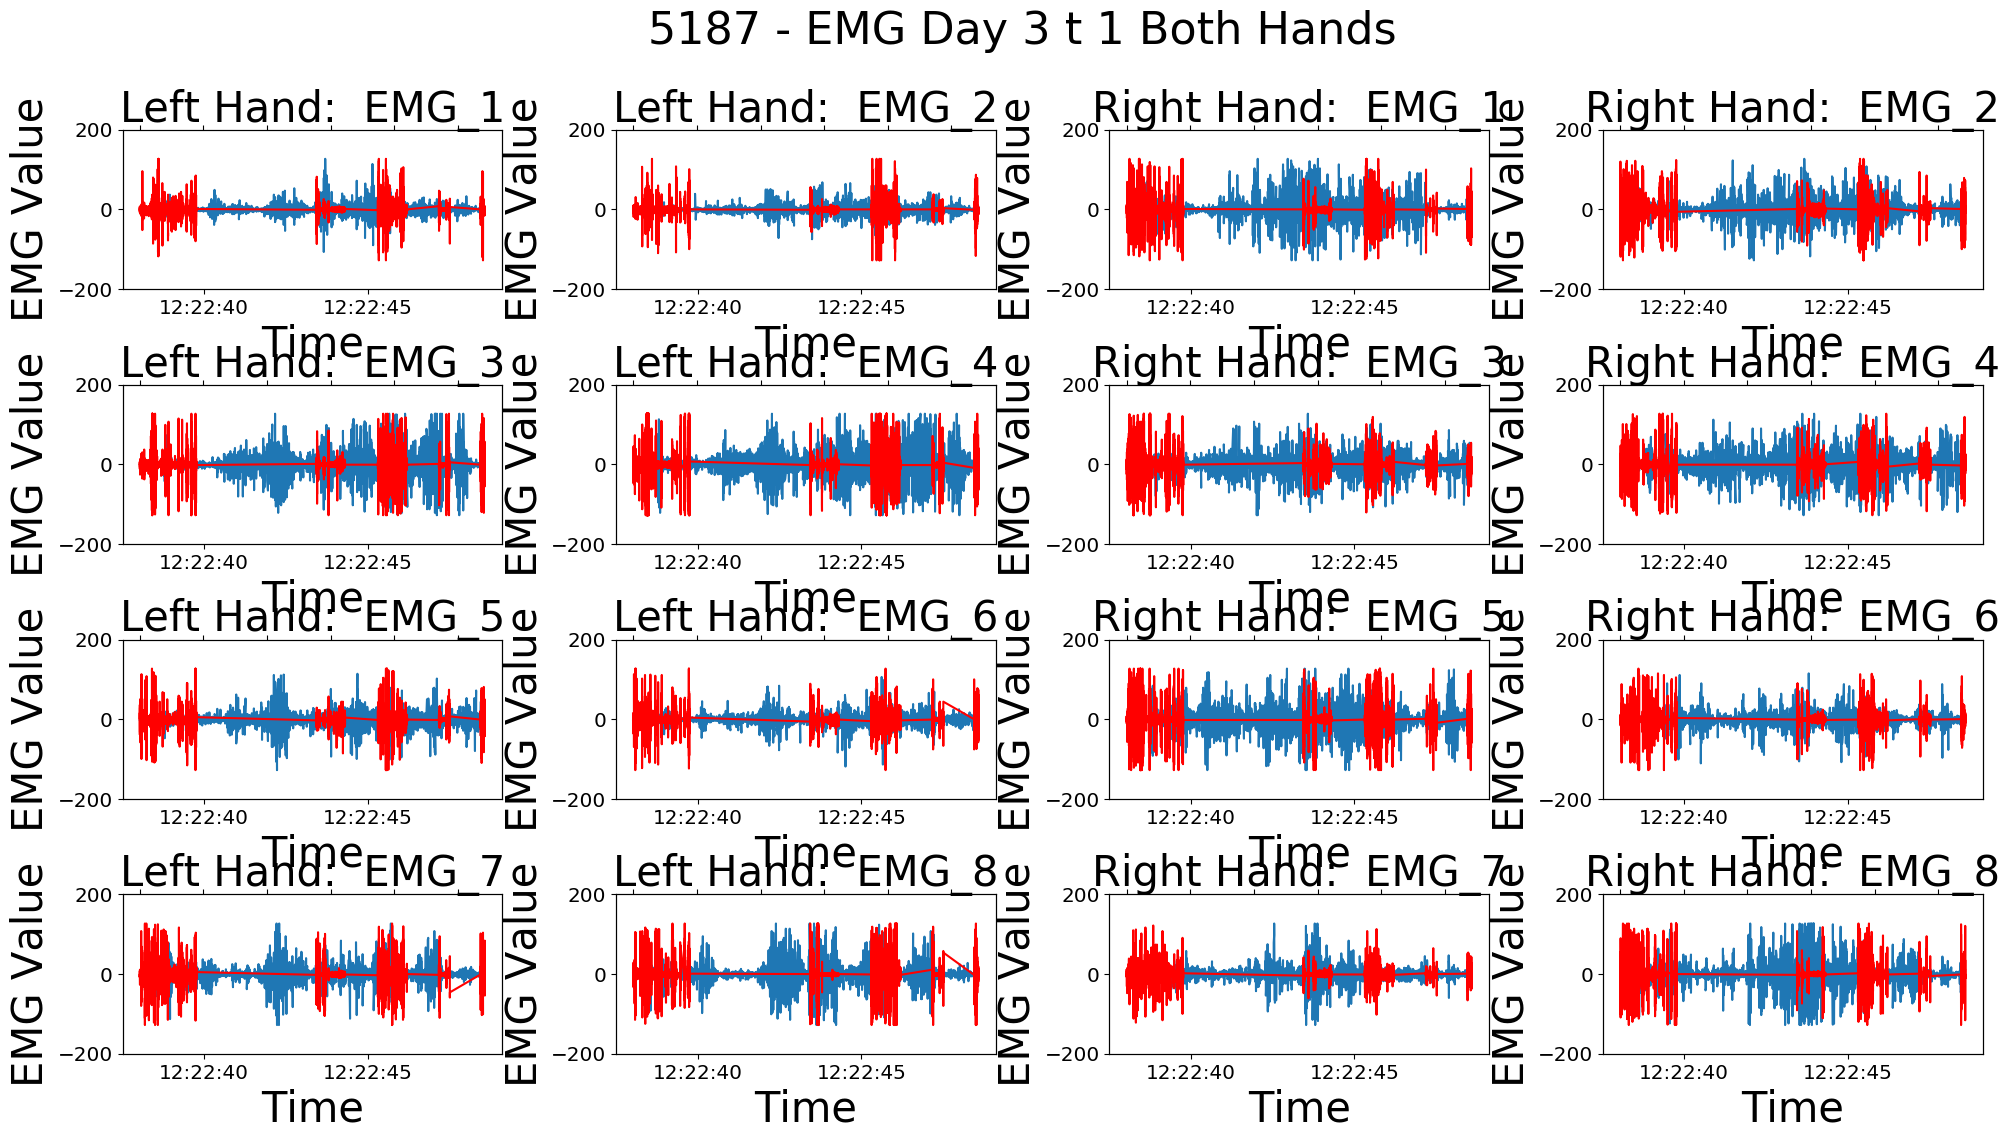
\includegraphics[width=\linewidth]{pictures/5187_EMG_Day3_t_1_average}
	\caption{Tourniquet EMG data with average in red}
	\label{fig:5187emgday3t1average}
\end{figure}

\subsection{Participant Generalizability Discussion}
\label{sec:Results:Generalizability:Discussion}

The combined dataset allowed the machine learning algorithms to train on several participants, each participant with different approaches to the procedures. The unique movements may all look similar, but the way participants grab and adjust tools can be different. 
The F1 score for the generalized population is close to the results generated for individual participants. The F1 score of the decision-tree algorithm for tying a tourniquet was on average 0.81 per participant and 0.74 across all participants. For wrapping a wound the F1 of the decision-tree algorithm was on average 0.90 per participant and 0.82 across all participants. Therefore, the algorithms are able to generalize across participants. The algorithms are also able to accurately detect a subset of procedures used inside an ambulance. While some procedures can be detected more accurately, others need improvements before the system can be deployed in real life scenarios.


\section{Discussion}
\label{sec:Results:Discussion}
The results clearly show that it is feasible to successfully recognize procedures performed by EMS personnel on patients using the Myo sensor. The results also show a high variance in accuracy depending on the algorithm and procedure. The comparison between the decision-tree, $k$-NN, SVM, and HMM algorithm highlight the strengths of the decision-tree algorithm. The algorithms were able to successfully detect the procedures both individually and over all participants.
\par $H_1$ hypothesized that CPR and Bag-valve-mask ventilation will have the highest accuracy for each machine learning algorithm, due to its unique movements. CPR and Bag-valve-mask ventilation had neither the highest F1 score for individual participants or for all participants. The result shows that more data preparation needs to take place in order to separate similar movements, such as dividing the procedures further into their task and training the algorithms on a task basis, while using the sequence of tasks to detect the procedure.
\par $H_2$ hypothesized that the recognition of a procedure through the sequence of fine-grained movements using a Hidden Markov Model will be more accurate than detection through training coarse-grained movement models. The HMM algorithm achieved the highest F1 score for Bag-Valve-Mask ventilation with the individual participants results. The overall participant generalizability placed the HMM algorithm third.
\par The F1 score for the HMM was expected to be significantly higher given its ability to detect data sequences. The results from training using individual participants and all participants show that the HMM placed second behind the decision-tree.
\par The F1 score of the SVM was lower than expected. Missing computing power for the large dataset resulted in limited ability to vary the parameters to improve the accuracy. 
\par The machine learning algorithms can be further improved by varying the parameters to a greater extent. The low performing SVM algorithm can be improved by varying the $gamma$ and $C$ value, and using a different kernel function.
\par The Hidden Markov Model algorithm can be further improved by optimizing selection of winners for all the models. Currently, the model with highest the log probability is picked as the correct result. The function can be improved by re-running the data, if the log probability of two models are withing a certain margin of error or printing out the probabilities to let the EMS personnel confirm the performed procedure after they return to their base.
\par Additionally, the Hidden Markov Model can be trained in a supervised manner. The hierarchical task analysis provides detail about the states included in a procedure. The states can be pre-defined and transition probabilities inferred. Furthermore, deep-learning algorithms, such as neural networks may achieve higher scores in case nonlinearity occurs in the dataset.
\par The generalizability can be further improved by collecting data from more participants. The data used in this thesis required participants to use specific hands for every procedure. Data, which includes left- and right-handed participants increases the generalizability.
\par The procedures represent those performed by EMS personnel on the way to the hospital inside of an ambulance. The movement of the ambulance introduces noise that can effect the accuracy of the machine learning algorithms. Future work can collect data in an ambulance simulation to improve real-life application.
\par Ambulances may include multiple EMS personnel, who can work on the patient simultaneously. The sensor has to be placed on all EMS personnel working on the patient in order to correctly identify the procedure. Future work can collect data from multiple participants at the same time and improve the machine learning algorithm to include data from more than two sensors.
\par Lastly, data from professionally trained EMS personnel may result in more consistent data, which may improve the score of all machine learning algorithms.
\par Overall, in order to use the technology in real world application, such as transmitting treatment information to a hospital in real-time requires a significantly higher detection accuracy. Unreliable treatment information can result in wrong preparation at the hospital, which may cause permanent injury or result in death. The procedure detection system needs to be further evaluated in real-life non-life threatening scenarios in order to obtain its effectiveness in improving communication between EMS personnel and hospital trauma staff. While there is room for improvement, the thesis is an initial step in detecting procedures inside of an ambulance.
%% LaTeX2e class for student theses
%% sections/conclusion.tex
%% 
%% Karlsruhe Institute of Technology
%% Institute for Program Structures and Data Organization
%% Chair for Software Design and Quality (SDQ)
%%
%% Dr.-Ing. Erik Burger
%% burger@kit.edu
%%
%% Version 1.3.2, 2017-08-01

\chapter{Conclusion}
\label{ch:Conclusion}

This thesis provided a novel approach to recognize CPR, bag-valve-mask ventilation, placing an oral airway, placing an IV tourniquet, and wrapping a head wound using data collected by the Myo and machine-learning algorithms. The five procedures were broken into their anatomical movements using hierarchical task analysis. The Myo sensor was chosen for its ability to sense most of the anatomical movements. Data from the Myo was processed and seven features were generated. The SVM, $k$-NN, and decision-tree machine learning algorithms were compared to Hidden Markov Models for every procedure. A user evaluation with ten participants was used to obtain the data necessary to train and evaluate the algorithms. The participants were trained in the procedures for two days, and data was collected on the third day. The Decision-tree achieved the highest F1 score and is feasible for inclusion into a system that automatically detects EMS procedures. The machine learning algorithms were applied to data from every individual participant and compared to data from all participants combined. The F1 score for the procedures were similar within a small margin and the data can therefore be considered generalizable.
\par Future work will be able to further segment the procedures to limit the detection to a specific task rather than the entire procedure. Through the series of tasks the procedure can then be implied. The use of artificial neural networks may also improve the detection accuracy and yield better results at detecting the subset of procedures. When higher detection results are achieved more procedures can be included in the detection system.
\par The EMS procedure detection system can already use the developed algorithms to assist EMS personnel in filling out paperwork by suggesting the detected procedure. The procedure detection system allows for faster paper work completion without any harm for the treatment of the patient.

%% --------------------
%% |   Bibliography   |
%% --------------------

%% Add entry to the table of contents for the bibliography
\printbibliography[heading=bibintoc]

%% ----------------
%% |   Appendix   |
%% ----------------
\appendix
%% LaTeX2e class for student theses
%% sections/apendix.tex
%% 
%% Karlsruhe Institute of Technology
%% Institute for Program Structures and Data Organization
%% Chair for Software Design and Quality (SDQ)
%%
%% Dr.-Ing. Erik Burger
%% burger@kit.edu
%%
%% Version 1.3.2, 2017-08-01


\iflanguage{english}
{\chapter{Appendix}}    % english style
{\chapter{Anhang}}      % german style
\label{chap:appendix}


%% -------------------
%% | Example content |
%% -------------------
\section{First Appendix Section}
\label{sec:appendix:FirstSection}
		
\setcounter{figure}{0}
		
\begin{figure} [ht]
  \centering
  \caption{A figure}
  \label{fig:anotherfigure}
\end{figure}


\dots
%% ---------------------
%% | / Example content |
%% ---------------------

\end{document}
